De nombreux phénomènes dépendent de plusieurs paramètres, par exemple le volume d'un gaz dépend de la température et de la pression; l'altitude $z$ d'un terrain dépend des coordonnées $(x,y)$ du lieu.

Dans les réseaux de neurones, les fonctions de plusieurs variables interviennent de deux manières :
\begin{itemize}
	\item lors de l'utilisation d'un réseau. C'est la partie la plus facile et la plus fréquente. On utilise un réseau déjà bien paramétré pour répondre à une question (Est-ce une photo de chat ? Tourner à droite ou à gauche ? Quel pion déplacer au prochain coup ?). La réponse est un calcul direct obtenu en évaluant une fonction de plusieurs variables. 
	
	\item lors de la paramétrisation du réseau. C'est la partie difficile et le but de ce cours. Quels paramètres choisir pour définir ce réseau afin qu'il réponde au problème ? Ces paramètres seront choisis comme minimum d'une fonction de plusieurs variables. Une des difficultés est qu'il peut y avoir des milliers de paramètres à gérer.
	
\end{itemize}




%%%%%%%%%%%%%%%%%%%%%%%%%%%%%%%%%%%%%%%%%%%%%%%%%%%%%%%%%%%%%%%%%%%%%
\section{Définition et exemples}

%--------------------------------------------------------------------
\subsection{Définition}


Nous allons étudier les fonctions de deux variables, mais aussi de trois variables et plus généralement de $n$ variables.
Ces fonctions sont donc de la forme 
$$f : \Rr^n \rightarrow \Rr$$
où $n$ est un entier naturel supérieur ou égal à $1$. 


Un élément de l'ensemble de départ est un vecteur de type  $x = (x_1,\ldots,x_n)$. À chacun de ces vecteurs, $f$ associe un nombre réel $f(x_1,\ldots,x_n)$. On pourrait aussi limiter l'ensemble de départ à une partie $E$ de $ \Rr^n$.



%--------------------------------------------------------------------
\subsection{Deux variables}

Lorsque $n=2$, on préfère noter les variables $(x,y)$ plutôt que $(x_1,x_2)$.
Voici quelques exemples.
\begin{exemple}{}{}
	
	\begin{itemize}
		\item $f(x,y) = 2x+3y^2+1$.
		\item $f(x,y) = \cos(xy)$.
		\item $f(x,y) = \sqrt{x^2+y^2}$. $f$ renvoie la distance entre un point $M(x,y)$ et l'origine $O(0,0)$.
		
		\myfigure{1}{
			\tikzinput{fig-fonctions-01}
		}
		
		\item L'équation physique $PV=nRT$ implique $T = \frac{1}{nR}PV$ :
		la température d'un gaz s'exprime en fonction de son volume et de la pression ($n$ et $R$ sont des constantes).
		\item La distance entre une droite fixée $\mathcal{D}$ d'équation $ax+by+c=0$ et un point $M(x_0,y_0)$ est donnée par une fonction de deux variables : $$d(x_0,y_0) = d(M,\mathcal{D}) = \frac{|ax_0+by_0+c|}{\sqrt{a^2+b^2}}.$$
		
		\myfigure{1}{
			\tikzinput{fig-fonctions-02}
		}
		
		
	\end{itemize}
\end{exemple}


%--------------------------------------------------------------------
\subsection{Trois variables}

\begin{exemple}{}{}
	
	\begin{enumerate}
		\item $f(x,y,z) = ax+by+cz+d$. Cette fonction $f$ est une fonction affine ($a,b,c,d$ sont des constantes).
		\item $f(x,y,z) = x^2+y^2+z^2$ qui donne la distance au carré entre un point $M(x,y,z)$ et l'origine $O(0,0,0)$.
		\item Le volume d'un cône à base rectangulaire dépend des longueurs des côtés $a$ et $b$ de la base et de la hauteur $h$ :
		$$V = f(a,b,h) = \frac13 abh.$$
		
		\myfigure{0.5}{
			\tikzinput{fig-fonctions-03}
		}
		
	\end{enumerate}
\end{exemple}


%--------------------------------------------------------------------
\subsection{$n$ variables}

\begin{exemple}{}{}
	
	\begin{enumerate}
		\item $f(x_1,\ldots,x_n) = a_1x_1+\cdots+a_nx_n+a_0$ une fonction affine (les $a_i$ sont des constantes).
		\item $f(x_1,\ldots,x_n) = \sqrt{(x_1-a_1)^2+\cdots+(x_n-a_n)^2}$ exprime la distance entre les points $M(x_1,\ldots,x_n)$ et $A(a_1,\ldots,a_n)$ dans $\Rr^n$.
	\end{enumerate}
\end{exemple}


%%%%%%%%%%%%%%%%%%%%%%%%%%%%%%%%%%%%%%%%%%%%%%%%%%%%%%%%%%%%%%%%%%%%%
\section{Graphe}

Le cas le plus simple, et déjà connu, est celui des fonctions d'une seule variable $f : \Rr \rightarrow \Rr$.  C'est l'ensemble de tous les points du plan de la forme $(x,f(x))$. Voici le graphe de la fonction $x \mapsto x\cos x$.

\myfigure{0.8}{
	\tikzinput{fig-fonctions-04}
} 



%--------------------------------------------------------------------
\subsection{Définition}





\begin{definition}{}{}
	Le \trouer{graphe} $\mathcal{G}_f$ d'une fonction de deux variables $f : \Rr^2 \to \Rr$ est  l'ensemble des points de $\Rr^3$ ayant pour coordonnées $(x,y,f(x,y))$, pour $(x,y)$ parcourant $\Rr^2$. Le graphe est donc :
	$$\mathcal{G}_f= \big\{ (x,y,z) \in \Rr^3 \mid (x,y)\in \Rr^2 \text{ et } z=f(x,y)\big\}.$$
\end{definition}

Dans le cas de deux variables, le graphe d'une fonction est une surface tracée dans l'espace.


\myfigure{0.7}{
	\tikzinput{fig-fonctions-05}
}


\begin{exemple}{}{}
	On souhaite tracer le graphe de la fonction définie par :
	$$f(x,y) = x  e^{-x^2-y^2}.$$
	
	On commence par tracer quelques points à la main :
	\begin{itemize}
		\item si $(x,y) = (0,0)$ alors $f(x,y) = f(0,0) = 0$ donc le point de coordonnées $(0,0,0)$ appartient au graphe.
		\item Comme $f(1,0) = 1/e$ alors le point de coordonnées $(1,0,1/e)$ appartient au graphe.
		\item Pour n'importe quel $y$, on a $f(0,y)=0$ donc la droite de l'espace d'équation ($x=0$ et $z=0$) est incluse dans le graphe.
		\item Notons $r = \sqrt{x^2+y^2}$ la distance entre le point de coordonnées $(x,y)$ et l'origine $(0,0)$ alors on a la formule $f(x,y) = x e^{-r^2}$. Pour un point éloigné de l'origine, $r$ est grand, donc  $e^{-r^2}$ est très petit, et $f(x,y)$ est très proche de $0$.
	\end{itemize}
	
	
	Voici différentes vues de ce graphe.
	
	\begin{center}
		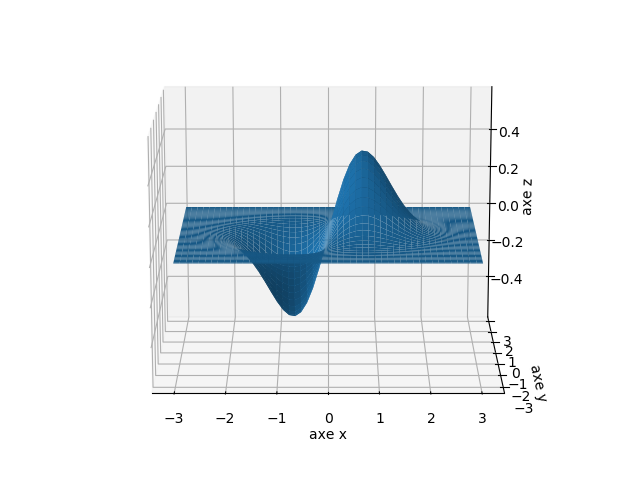
\includegraphics[scale=\myscale,scale=0.5]{figures/fonctions-surface-1a}
		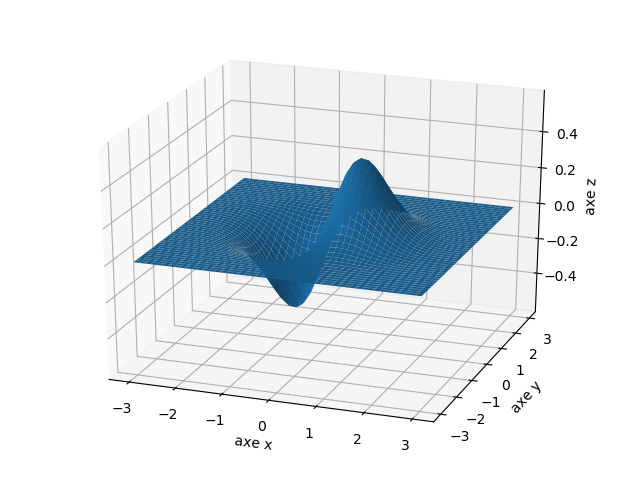
\includegraphics[scale=\myscale,scale=0.5]{figures/fonctions-surface-1b}
		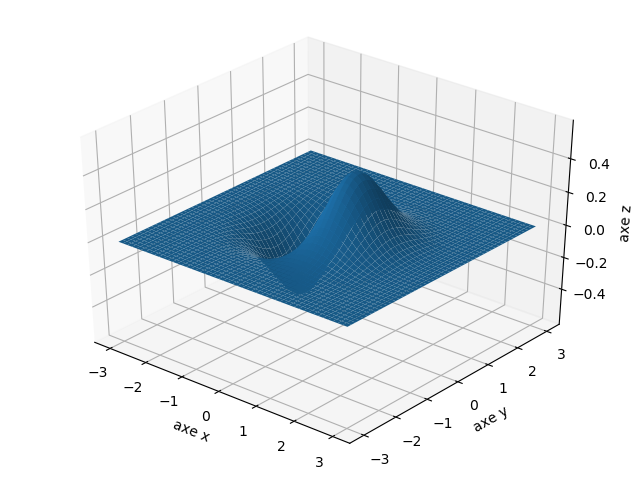
\includegraphics[scale=\myscale,scale=0.5]{figures/fonctions-surface-1c}
		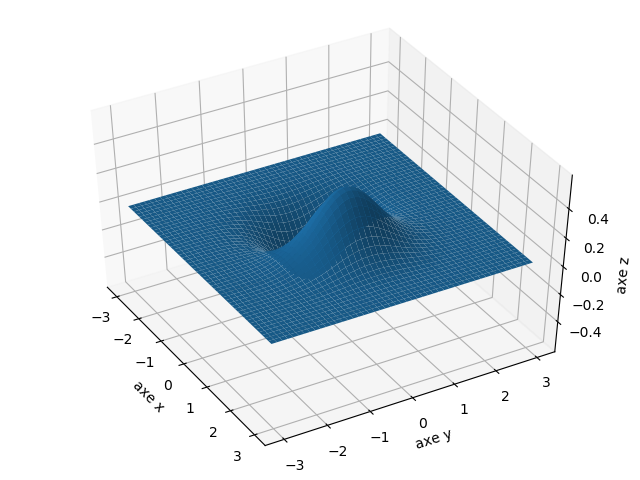
\includegraphics[scale=\myscale,scale=0.5]{figures/fonctions-surface-1d}
	\end{center}
	
	%  fichier python 'fonctions-surface-1.py'
\end{exemple}


%--------------------------------------------------------------------
\subsection{Tranches}

Afin de tracer le graphe d'une fonction de deux variables, on peut découper la surface en \og{}tranches\fg{}.
On fixe par exemple une valeur $y_0$ et on trace dans le plan $(xOz)$ le graphe de la fonction d'une variable  
$$f_{|y_0} : x\mapsto f(x,y_0).$$
Géométriquement, cela revient à tracer l'intersection du graphe de $f$ et du plan d'équation $(y=y_0)$.
On recommence pour plusieurs valeurs de $y_0$, ce qui nous donne des tranches du graphe de $f$ et nous donne une bonne idée du graphe complet de $f$.

On peut faire le même travail en fixant des valeurs $x_0$ avec les fonctions :
$$f_{|x_0} : y \mapsto f(x_0,y).$$


\begin{exemple}{}{}
	On souhaite tracer le graphe de la fonction définie par :
	$$f(x,y) = x \sin(y).$$
	
	\begin{center}
		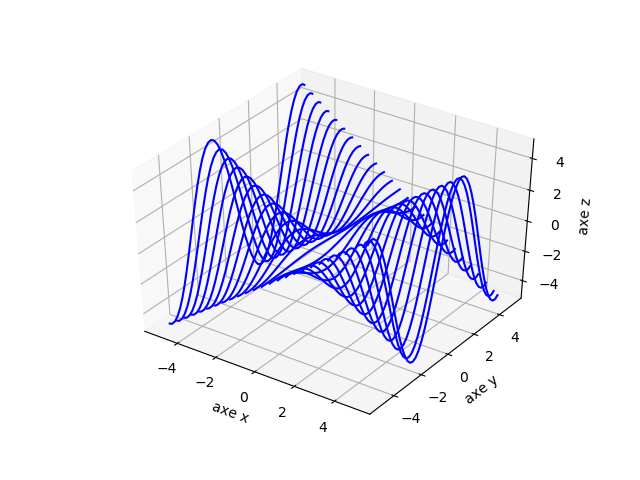
\includegraphics[scale=\myscale,scale=0.5]{figures/fonctions-surface-2a}
		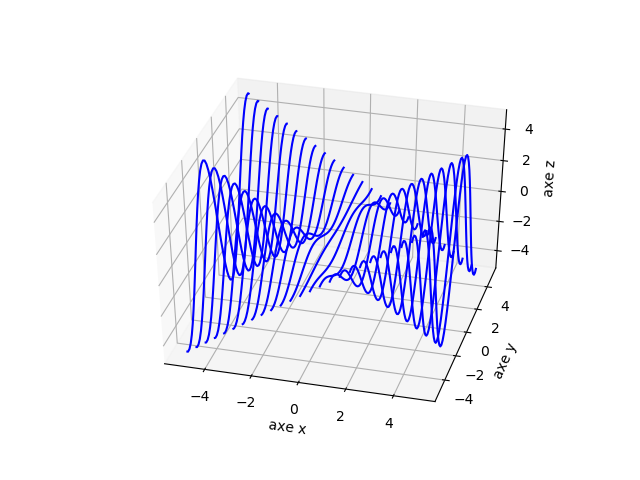
\includegraphics[scale=\myscale,scale=0.5]{figures/fonctions-surface-2b}
		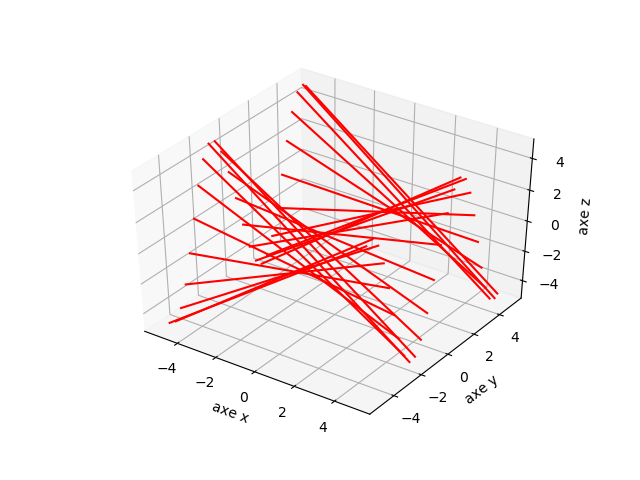
\includegraphics[scale=\myscale,scale=0.5]{figures/fonctions-surface-2c}
		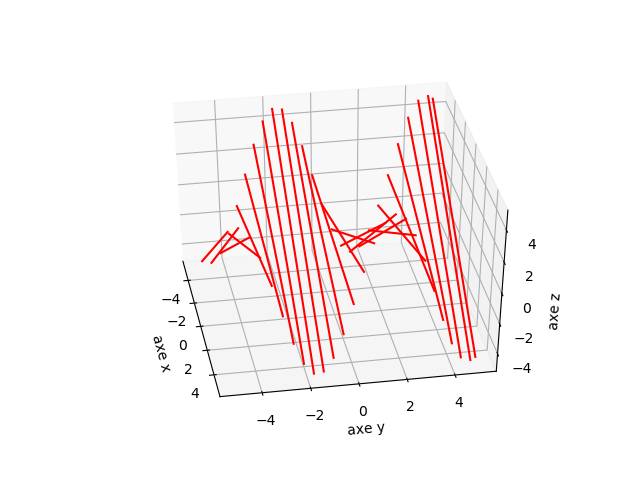
\includegraphics[scale=\myscale,scale=0.5]{figures/fonctions-surface-2d}
		
		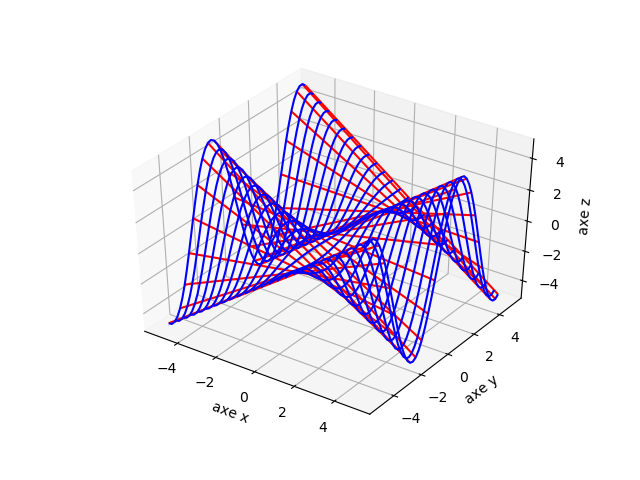
\includegraphics[scale=\myscale,scale=0.7]{figures/fonctions-surface-2e}
	\end{center}
	
	\couleurnb{En bleu}{En haut} les tranches pour lesquelles $x$ est constant (deux points de vue), \couleurnb{en rouge}{au milieu} les tranches pour lesquelles $y$ est constant (deux points de vue). Lorsque l'on rassemble les tranches (à $x$ constant et à $y$ constant), on reconstitue la surface (dernière figure). 
	
	% voir fichier python 'fonctions-surface-2.py'
	
\end{exemple}


%--------------------------------------------------------------------
\subsection{Minimum, maximum}

Pour des fonctions de deux variables (ou plus) il existe une notion de minimum et de maximum.


\begin{definition}{}{}
	\index{minimum!local}
	\index{minimum!global}
	Soit $f : \Rr^2 \to \Rr$ une fonction.
	\begin{itemize}
		\item $f$ atteint un \trouer{minimum global} en $(x_0,y_0) \in \Rr^2$ si
		pour tout $(x,y) \in \Rr^2$, on a $f(x,y) \ge f(x_0,y_0)$.
		
		\item $f$ atteint un \trouer{minimum local} en $(x_0,y_0) \in \Rr^2$ si
		il existe un intervalle ouvert $I$ contenant $x_0$ et un intervalle ouvert $J$ contenant $y_0$  tels que 
		pour tout $(x,y) \in I \times J$, on a $f(x,y) \ge f(x_0,y_0)$. 
	\end{itemize}
\end{definition}



\begin{exemple}{}{}
	Voici l'exemple d'une fonction qui admet deux minimums locaux. L'un est aussi un minimum global. Elle admet un maximum local qui est aussi global.
	
	\begin{center}
		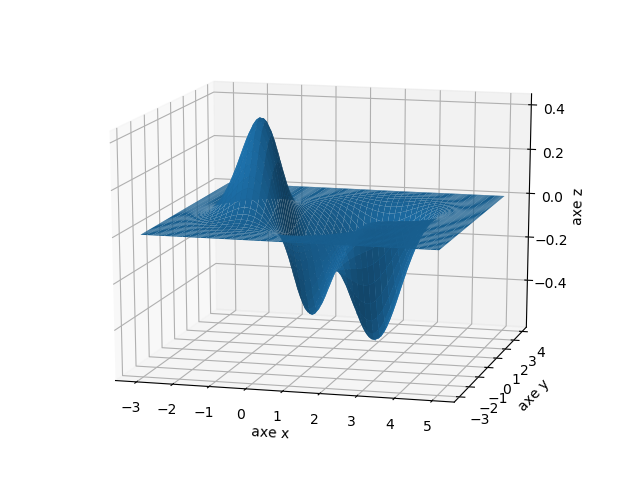
\includegraphics[scale=\myscale,scale=0.7]{figures/fonctions-surface-3}
	\end{center}
	
	% voir fichier python 'fonctions-surface-3.py'
	
\end{exemple}


Trouver les bons paramètres d'un réseau de neurones nous amènera à trouver le minimum d'une fonction de plusieurs (et même de centaines de) variables. Voyons un exemple en deux variables.
\begin{exemple}{}{}
	Étant donnés trois points $A(1,2)$, $B(3,5)$ et $C(6,1)$, il s'agit de trouver un point $M(x,y)$ qui \og{}approche au mieux\fg{} ces trois points. Il faut expliciter une fonction à minimiser pour définir correctement le problème. Nous décidons de prendre la somme des carrés des distances.
	
	
	\myfigure{1}{
		\tikzinput{fig-fonctions-06}
	}
	
	Il s'agit donc de minimiser la fonction $f$ suivante, qui correspond à une fonction distance (aussi appelée fonction erreur ou bien fonction coût) :
	$$f(x,y) = MA^2+MB^2+MC^2 = 
	(x-1)^2+ (y-2)^2 + (x-3)^2 + (y-5)^2 + (x-6)^2 + (y-1)^2.$$
	En développant on trouve :
	$$f(x,y) = 3x^2 + 3y^2 - 20x - 16y + 76.$$
	
	Le graphe de $f$ nous suggère qu'il existe un unique minimum qui est le minimum global de $f$. 
	Par recherche graphique ou par les méthodes décrites dans la section suivante, on trouverait une solution approchée. En fait la solution géométrique exacte est l'isobarycentre des points (autrement dit le centre de gravité du triangle $ABC$), ainsi :
	$$(x_0,y_0) = \left(\frac{10}{3},\frac83\right) \simeq (3.33,2.66)$$
	pour lequel $f$ atteint son minimum $z_0 = f(x_0,y_0) = \frac{64}{3} \simeq 21.33$.
	
	\begin{center}
		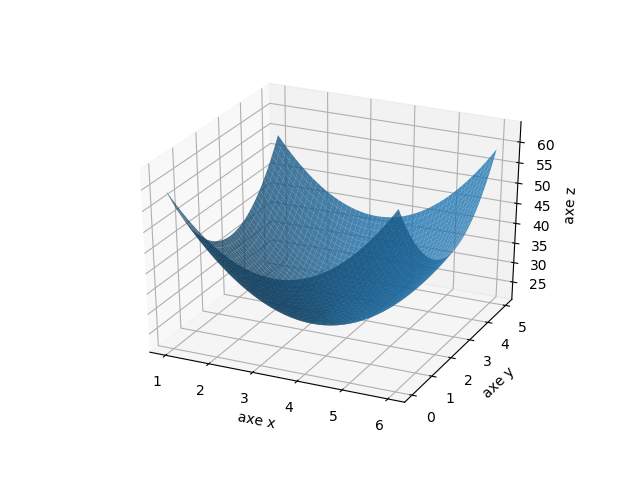
\includegraphics[scale=\myscale,scale=0.7]{figures/fonctions-surface-4}
	\end{center}
	
	% voir fichier python 'fonctions-surface-4.py'
	% voir fichier sage 'fonctions-surface-4.sage' pour résolution exacte
	
	Le point qui convient le mieux à notre problème et en lequel notre fonction distance est minimale est donc le point de coordonnées $(\frac{10}{3},\frac83)$. Attention, un autre choix de la fonction distance $f$ pourrait conduire à une autre solution (voir l'exemple de la prochaine section).
	
	\myfigure{1}{
		\tikzinput{fig-fonctions-07}
	}
	
	
\end{exemple}

%--------------------------------------------------------------------
\subsection{Recherche élémentaire d'un minimum}


Voici trois techniques pour trouver les valeurs approchées des coordonnées du point en lequel une fonction de plusieurs variables atteint son minimum. Ces techniques sont valables quelque soit le nombre de variables même si ici elles ne sont décrites que dans le cas de deux variables. 

\textbf{Recherche sur une grille.} On calcule $f(x,y)$ pour $(x,y)$ parcourant une grille. On retient le point $(x_0,y_0)$ en lequel $z_0=f(x_0,y_0)$ est le plus petit. Si on le souhaite, on peut affiner la grille autour de ce point, en diminuant le pas $\epsilon$ pour améliorer l'approximation. C'est une technique qui demande $N^2$ calculs pour une grille de largeur $N$ (et même $N^n$ pour une fonction de $n$ variables) ce qui peut être énorme.

\myfigure{0.5}{
	\tikzinput{fig-fonctions-08}
}


\textbf{Recherche au hasard.} Cela peut sembler incongru mais choisir quelques coordonnées $(x,y)$ au hasard, calculer chaque valeur $z=f(x,y)$ et comme auparavant retenir le point $(x_0,y_0)$ correspondant au $z_0$ minimal n'est pas ridicule !
Un ordinateur peut tester plusieurs millions de points en quelques secondes. Bien sûr il y a de fortes chances de ne trouver qu'une solution approchée. C'est aussi une technique que l'on retrouvera plus tard : partir d'un point au hasard pour ensuite construire une suite de points convergeant vers un minimum. Et si cela n'est pas concluant, il faudra repartir d'un autre point tiré au hasard.

\bigskip

\textbf{Recherche par tranche.} 
L'idée est de se ramener à des fonctions d'une seule variable. En effet, 
pour les fonctions d'une variable, on sait qu'il faut chercher les minimums là où la dérivée s'annule.

On part d'une valeur $x_0$ (au hasard !). On cherche le minimum sur la tranche $x=x_0$, c'est-à-dire que l'on cherche le minimum de la fonction d'une variable $y \mapsto f(x_0,y)$. On trouve une valeur $y_0$ qui réalise un minimum. On change alors de direction en étudiant maintenant la tranche $y=y_0$ (pour le $y_0$ que l'on vient d'obtenir), on obtient l'abscisse $x_1$ du minimum de la fonction d'une variable $x \mapsto f(x,y_0)$. On recommence depuis le début à partir de ce $x_1$. On obtient ainsi une suite de points $(x_i,y_i)$ avec des valeurs $z_i=f(x_i,y_i)$ de plus en plus petites. On peut espérer tendre vers un minimum. %que $(x_i,y_i)$ tendent vers un minimum.


\myfigure{1}{
	\tikzinput{fig-fonctions-09}
}

Sur la figure ci-dessus, on part d'une tranche \couleurnb{(en bleu) }{}choisie au hasard, donnée par $x=x_0$. Cette tranche définit le graphe d'une fonction d'une variable. On se déplace sur cette courbe jusqu'à atteindre le minimum de cette tranche, en une valeur $y_0$. On considère la tranche perpendiculaire donnée par $y=y_0$. On se déplace sur la courbe \couleurnb{rouge }{}jusqu'à atteindre le minimum de cette tranche, en une valeur $x_1$. On pourrait continuer avec une nouvelle tranche \couleurnb{bleue }{}$x=x_1$, etc.

\bigskip

Les descriptions données ici sont assez informelles, d'une part parce qu'il est difficile d'énoncer des théorèmes qui garantissent d'atteindre un minimum local et d'autre part parce qu'aucune technique ne garantit d'atteindre un minimum global. Lorsque l'on étudiera le gradient, nous obtiendrons une méthode plus efficace.

\begin{exemple}{}{}
	On reprend le problème précédent, à savoir trouver un point $M$ qui approche au mieux les trois points $A$, $B$ et $C$, mais cette fois on choisit la \og{}vraie\fg{} distance comme fonction d'erreur :
	$$g(x,y) = MA+MB+MC = 
	\sqrt{(x-1)^2+ (y-2)^2} + \sqrt{(x-3)^2 + (y-5)^2} + \sqrt{(x-6)^2 + (y-1)^2}.$$
	On applique ces trois techniques pour chercher le minimum de $g$ en se limitant au carré $[0,6]\times[0,6]$.
	
	\begin{enumerate}
		
		\item Avec une grille $N\times N$. Par exemple pour $N=100$, on évalue $g$ en $10\,000$ points. On trouve $(x_{\min},y_{\min}) \simeq (2.91,2.97)$ pour une valeur $z_{\min} \simeq 7.84$. 
		
		\item Avec un tirage aléatoire de $1000$ points, on trouve par exemple :
		$(x_{\min},y_{\min}) \simeq (2.88,2.99)$ et $z_{\min} \simeq 7.84$. Le résultat est similaire à la méthode précédente, bien qu'on ait effectué $10$ fois moins de calculs.
		
		\item Par les tranches. On part de la tranche $(x=0)$. On pose $x_0=0$, la fonction à étudier
		est donc 
		$$g_{|x_0}(y) = \sqrt{1 + (y-2)^2} + \sqrt{9 + (y-5)^2} + \sqrt{36 + (y-1)^2}.$$
		C'est une fonction de la seule variable $y$ pour laquelle on possède des techniques efficaces de recherche de minimum.
		On trouve que le minimum de $g_{|x_0}$ est atteint en $y_0 \simeq 2.45$.
		On recommence avec cette fois la tranche $(y = y_0)$ et on cherche le minimum de la fonction $g_{|y_0}(x) = g(x,y_0)$. On trouve que cette fonction atteint son minimum en $x_1 \simeq 2.84$. 
		On recommence ce processus jusqu'à atteindre la précision souhaitée.
		Ainsi en $5$ étapes on obtient une valeur approchée assez précise du minimum 
		$(x_{\min},y_{\min}) \simeq (2.90579,2.98464)$ et $z_{\min} \simeq 7.83867$.
		
		
	\end{enumerate}
\end{exemple}

La première conclusion à tirer de ce qui précède est que pour résoudre un problème il faut définir correctement une fonction d'erreur, c'est-à-dire celle que l'on cherche à minimiser. La solution trouvée dépend de cette fonction d'erreur choisie. 
Enfin, la méthode des tranches est une méthode efficace pour trouver un minimum d'une fonction, mais nous en découvrirons une encore meilleure en utilisant le gradient.


%%%%%%%%%%%%%%%%%%%%%%%%%%%%%%%%%%%%%%%%%%%%%%%%%%%%%%%%%%%%%%%%%%%%%
\section{Lignes de niveau}

\index{lignes de niveau}

%--------------------------------------------------------------------
\subsection{Définition}

\begin{definition}{}{}
	Soit $f : \Rr^2 \to \Rr$ une fonction de deux variables. 
	La \trouer{ligne de niveau} $z=c\in \Rr$ est l'ensemble de tous les points $(x,y)$ vérifiant $f(x,y)=c$ :
	$$L_c =\big\{(x,y)\in \Rr^2 \mid f(x,y)=c \big\}.$$
\end{definition}

La ligne de niveau $c$ est une courbe du plan $\Rr^2$. 

On peut aussi définir une \trouer{courbe de niveau}, c'est l'ensemble des points de l'espace obtenus comme intersection du graphe $\mathcal{G}_f$ et du plan $z=c$ qui est horizontal et \og{}d'altitude\fg{} $c$. Ce sont donc tous les points $(x,y,f(x,y))$ avec $f(x,y)=c$. On obtient la courbe de niveau en translatant la ligne de niveau d'une altitude $c$.



\begin{exemple}{}{}
	Soit $f : \Rr^2 \to \Rr$ définie par $f(x,y)=x^2+y^2$. 
	
	\begin{itemize}
		\item Si $c<0$, la ligne de niveau $L_c$ est vide (aucun point n'est d'altitude négative).
		\item Si $c=0$, la ligne de niveau $L_0$ se réduit à $\{(0,0)\}$.
		\item Si $c>0$, la ligne de niveau $L_c$  est le cercle du plan de centre $(0,0)$ et de rayon $\sqrt{c}$. On \og{}remonte\fg{} $L_c$ à l'altitude $z=c$ : la courbe de niveau est alors le cercle horizontal de l'espace de centre $(0,0,c)$ et de rayon $\sqrt{c}$. 
	\end{itemize}
	
	Le graphe est alors une superposition de cercles horizontaux de l'espace de centre $(0,0,c)$ et de rayon $\sqrt{c}$, $c>0$.     
	
	Ci-dessous : (a) la surface, (b) $5$ courbes de niveau, (c) $10$ courbes de niveau, (d) les lignes de niveau dans le plan.
	\begin{center}
		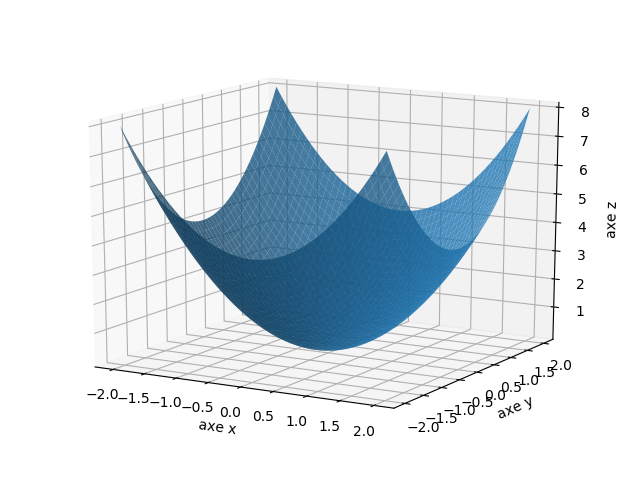
\includegraphics[scale=\myscale,scale=0.5]{figures/fonctions-niveau-1a}
		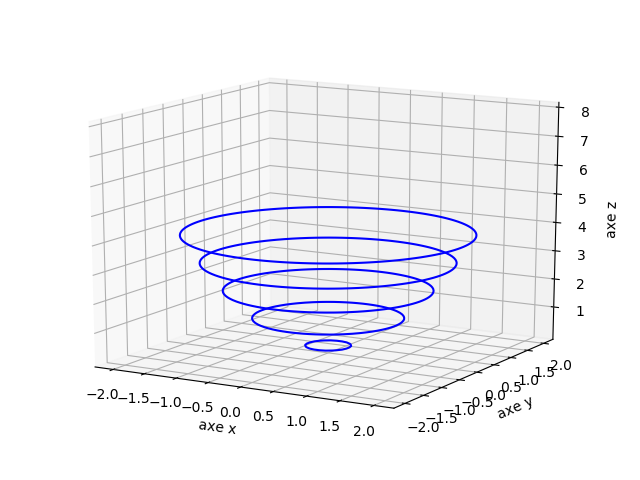
\includegraphics[scale=\myscale,scale=0.5]{figures/fonctions-niveau-1b}
		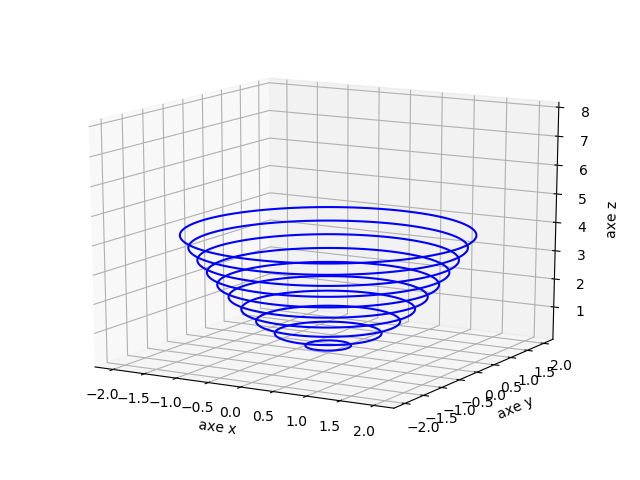
\includegraphics[scale=\myscale,scale=0.5]{figures/fonctions-niveau-1c}
		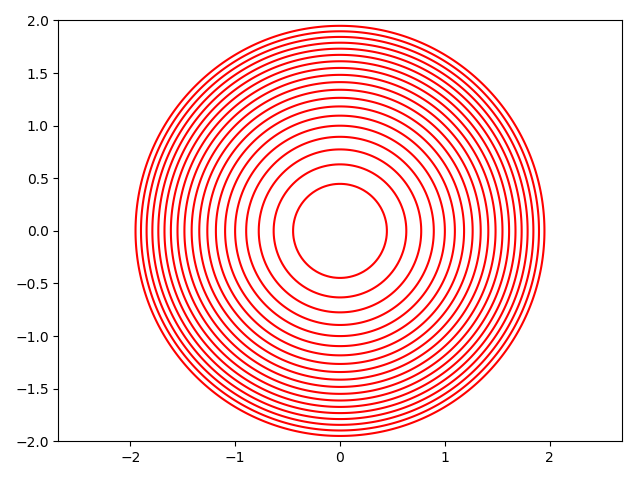
\includegraphics[scale=\myscale,scale=0.5]{figures/fonctions-niveau-1d}
	\end{center}
	
	% dessins 3d voir 'fonctions-niveau-1.py'
	
\end{exemple}


%--------------------------------------------------------------------
\subsection{Exemples}

\begin{exemple}{}{}
	Sur une carte topographique, les lignes de niveau représentent les courbes ayant la même altitude. 
	\begin{center}
		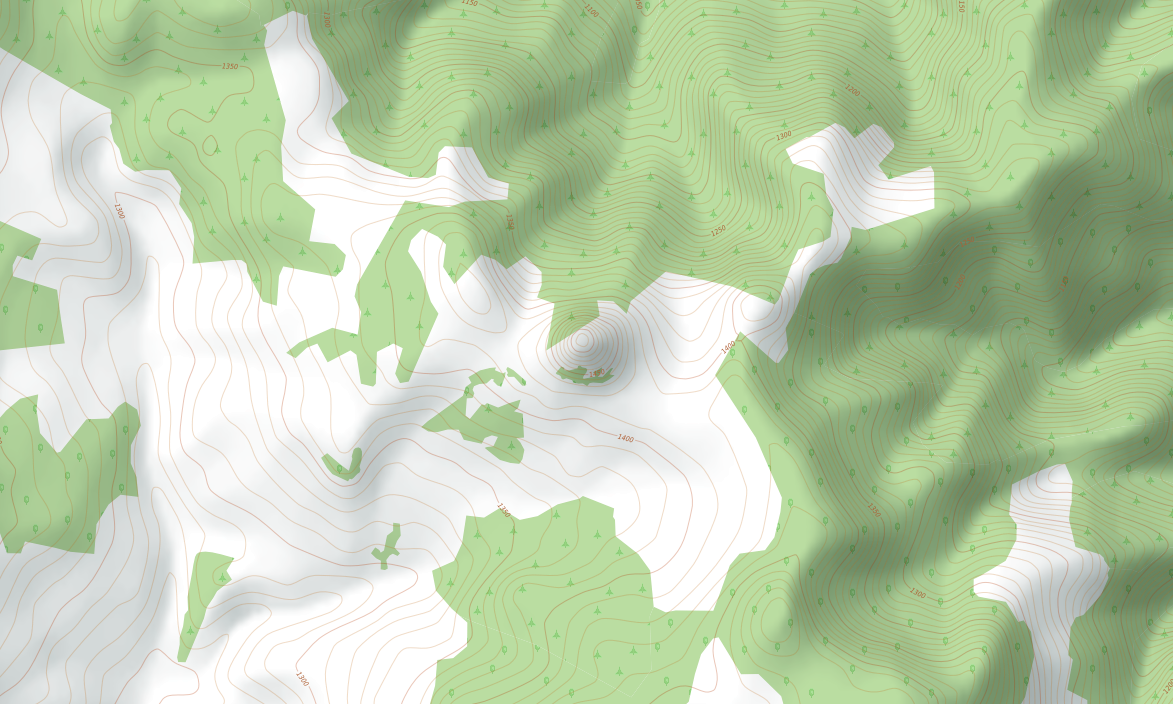
\includegraphics[scale=0.3]{figures/fig-fonctions-topo}
	\end{center}
	\begin{itemize}
		\item Ici, une carte \emph{Open Street Map} avec au centre le mont Gerbier de Jonc (source de la Loire, 1551 m). 
		\item Les lignes de niveau correspondent à des altitudes équidistantes de $10$ m (par exemple, pour $c=1400$, $c=1410$, $c=1420$\ldots).
		\item Lorsque les lignes de niveau sont très espacées, le terrain est plutôt plat ; lorsque les lignes sont rapprochées le terrain est pentu.
		\item Par définition, si on se promène en suivant une ligne de niveau, on reste toujours à la même altitude !
	\end{itemize}
\end{exemple}



\begin{exemple}{}{}
	Voici le graphe et les lignes de niveau de la fonction $f : \Rr^2 \to \Rr$ définie par
	$$f(x,y) = \frac{\sin(r^2-x)}{r}+1 \quad \text{ où } r = \sqrt{x^2+y^2}.$$
	
	\begin{center}
		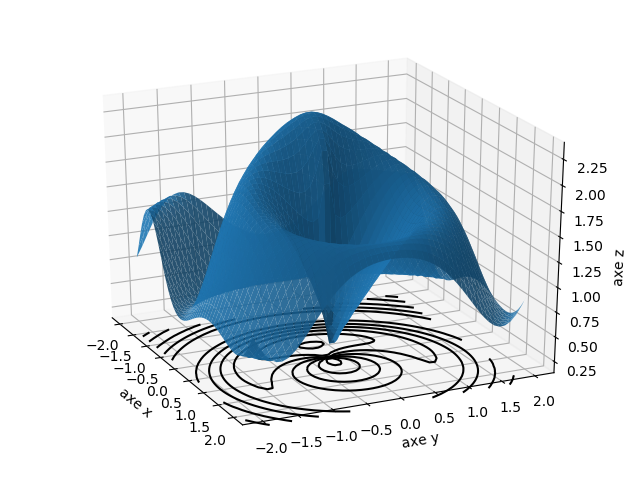
\includegraphics[scale=\myscale,scale=0.5]{figures/fonctions-niveau-2a}
		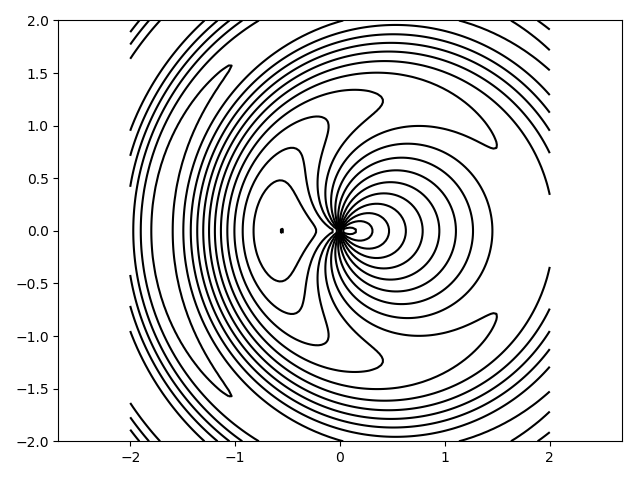
\includegraphics[scale=\myscale,scale=0.5]{figures/fonctions-niveau-2b}
	\end{center}
	% voir 'fonctions-niveau-2.py'
	
	
\end{exemple} 


%--------------------------------------------------------------------
\subsection{Surfaces quadratiques}

Ce sont des exemples à bien comprendre car ils seront importants pour la suite du cours.

\begin{exemple}{}{}
	$$f(x,y) = \frac{x^2}{a^2} + \frac{y^2}{b^2}-1$$
	
	
	
	\begin{itemize}
		\item Les tranches sont des paraboles.
		\item Les lignes de niveau sont des ellipses.
		\item Le graphe est donc un \trouer{paraboloïde elliptique}.
	\end{itemize}
	
	Ci-dessous : (a) la surface, (b) les tranches avec $x$ constant, (c) les tranches avec $y$ constant, (d) les courbes de niveau, (e) les lignes de niveau dans le plan.
	
	\begin{center}
		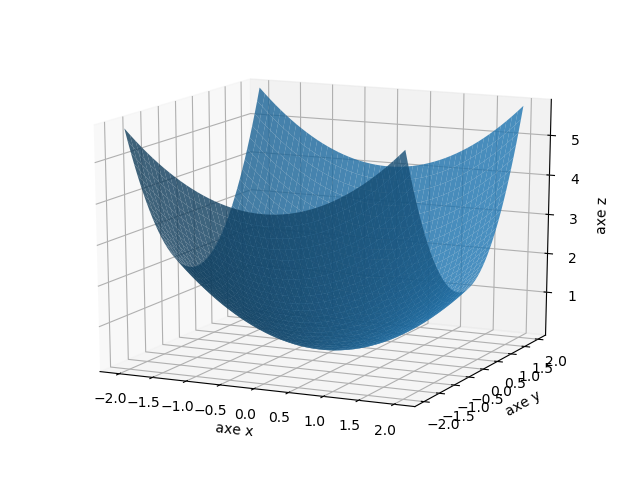
\includegraphics[scale=\myscale,scale=0.5]{figures/fonctions-quadra-1a}
		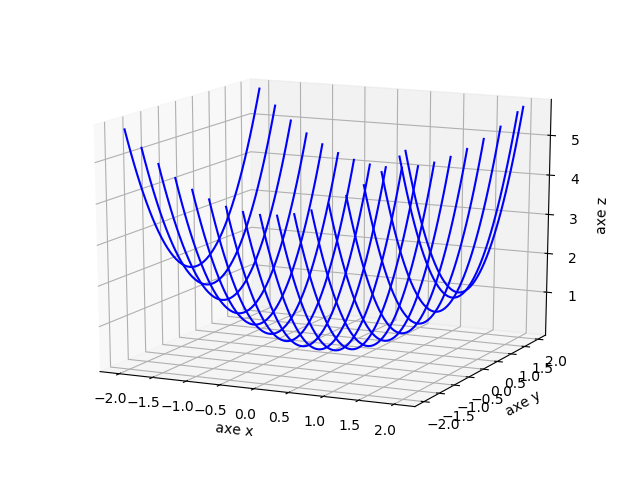
\includegraphics[scale=\myscale,scale=0.5]{figures/fonctions-quadra-1b}
		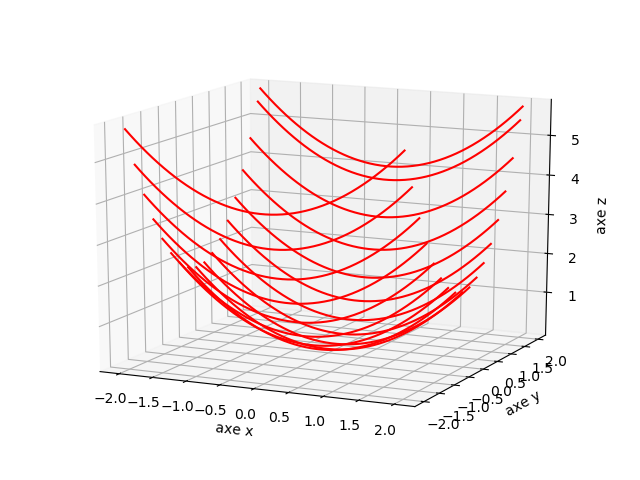
\includegraphics[scale=\myscale,scale=0.5]{figures/fonctions-quadra-1c}
		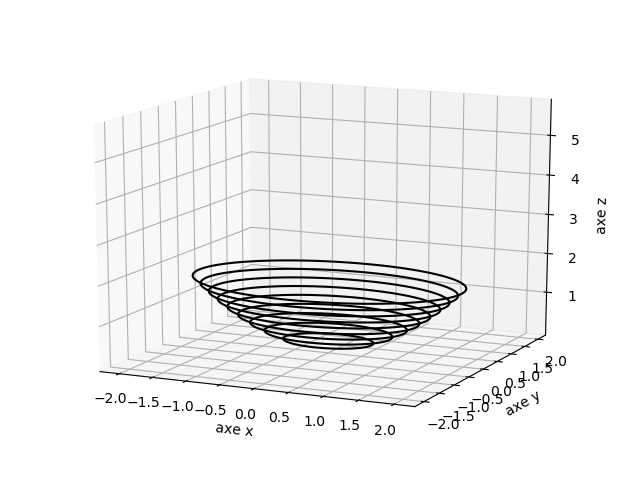
\includegraphics[scale=\myscale,scale=0.5]{figures/fonctions-quadra-1d}
		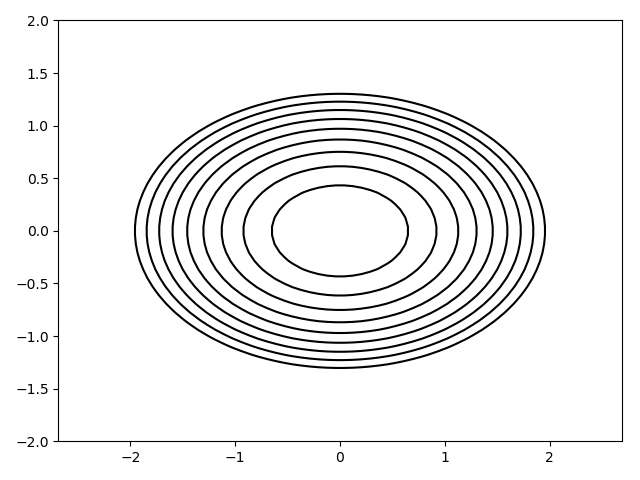
\includegraphics[scale=\myscale,scale=0.5]{figures/fonctions-quadra-1e}
	\end{center}
	
	% dessins 3d voir 'fonctions-quadra-1.py' 
	
\end{exemple}


\begin{exemple}{}{}
	$$f(x,y) = x^2$$
	
	
	
	\begin{itemize}
		\item Les tranches obtenues en coupant selon des plans $y=y_0$ sont des paraboles. Dans l'autre direction, ce sont des droites.
		\item Les lignes de niveau sont des droites.
		\item Le graphe est donc un \trouer{cylindre parabolique}.
	\end{itemize}
	
	Ci-dessous : (a) la surface, (b) les tranches avec $x$ constant, (c) les tranches avec $y$ constant, (d) les courbes de niveau, (e) les lignes de niveau dans le plan.
	\begin{center}
		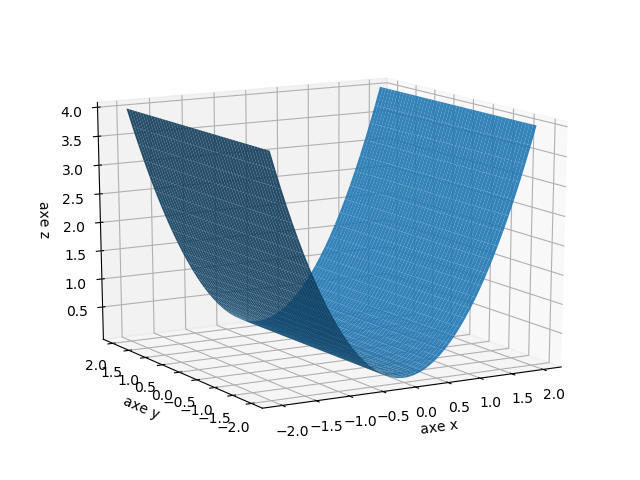
\includegraphics[scale=\myscale,scale=0.5]{figures/fonctions-quadra-2a}
		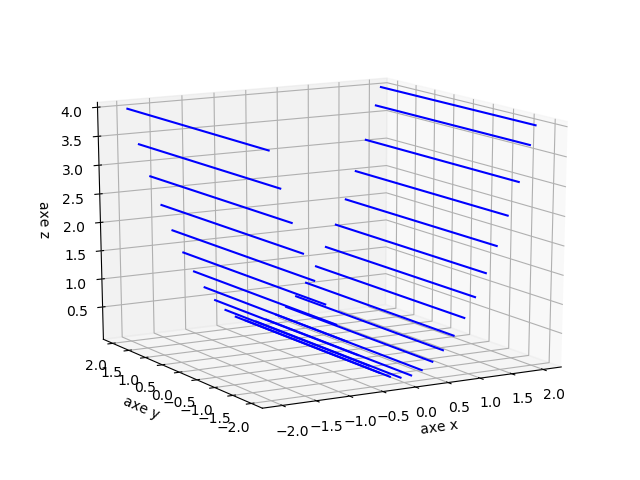
\includegraphics[scale=\myscale,scale=0.5]{figures/fonctions-quadra-2b}
		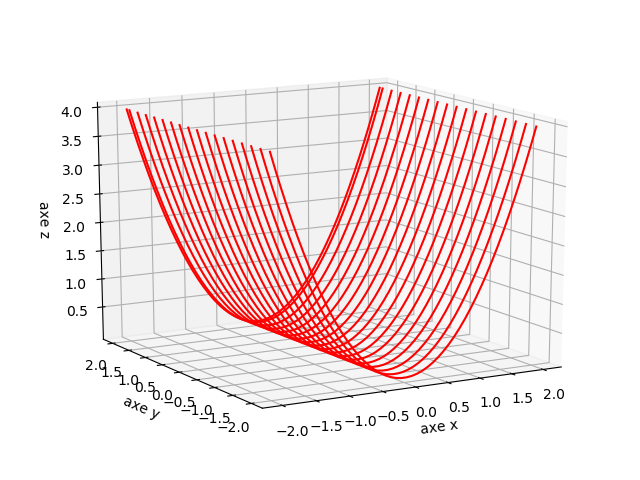
\includegraphics[scale=\myscale,scale=0.5]{figures/fonctions-quadra-2c}
		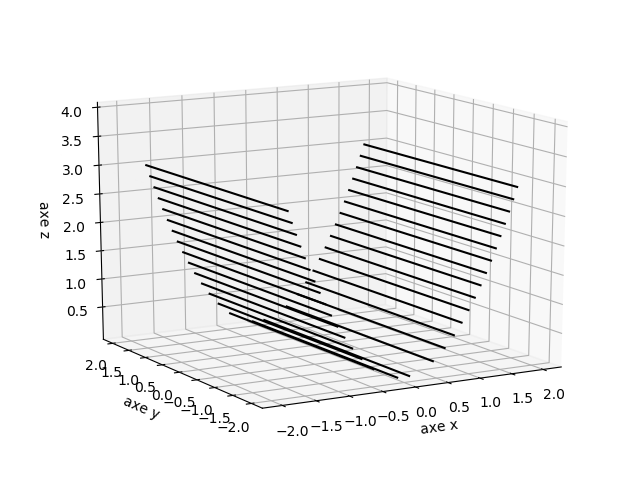
\includegraphics[scale=\myscale,scale=0.5]{figures/fonctions-quadra-2d}
		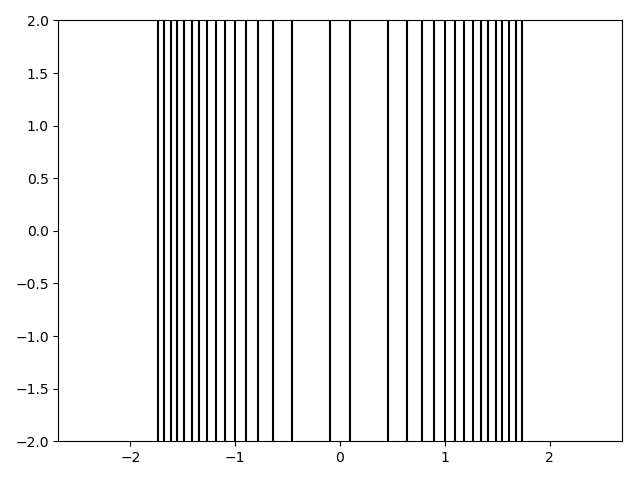
\includegraphics[scale=\myscale,scale=0.5]{figures/fonctions-quadra-2e}
	\end{center}
	
	% dessins 3d voir 'fonctions-quadra-2.py' 
	
	
\end{exemple}


\begin{exemple}{}{}
	$$f(x,y) = x^2-y^2$$
	
	
	\begin{itemize}
		\item Les tranches sont des paraboles, tournées vers le haut ou vers le bas selon la direction de la tranche.
		\item Les lignes de niveau sont des hyperboles.
		\item Le graphe est donc un \trouer{paraboloïde hyperbolique} que l'on appelle aussi la \trouer{selle de cheval}\index{point-selle}.
		\item Un autre nom pour cette surface est un \trouer{col} (en référence à un col en montagne). 
		En effet le point $(0,0,0)$, est le point de passage le moins haut pour passer d'un versant à l'autre de la montagne. 
	\end{itemize}
	
	Ci-dessous : (a) la surface, (b) les tranches avec $x$ constant, (c) les tranches avec $y$ constant, (d) les courbes de niveau, (e) les lignes de niveau dans le plan (en pointillé les lignes de niveau négatif).
	\begin{center}
		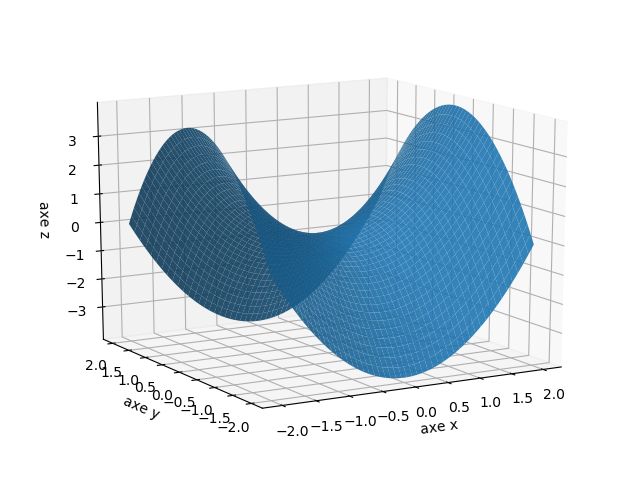
\includegraphics[scale=\myscale,scale=0.5]{figures/fonctions-quadra-3a}
		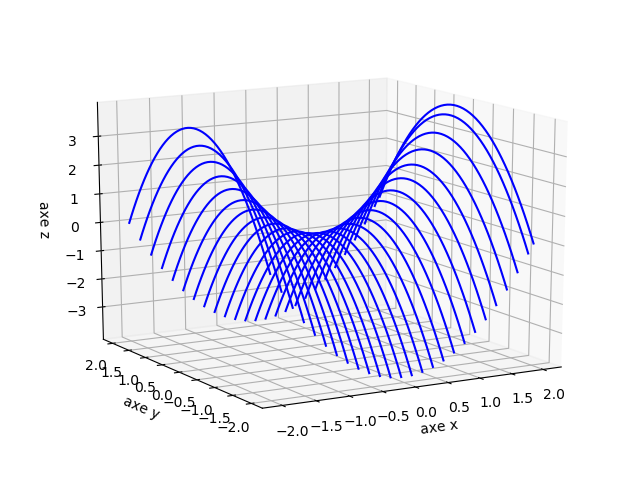
\includegraphics[scale=\myscale,scale=0.5]{figures/fonctions-quadra-3b}
		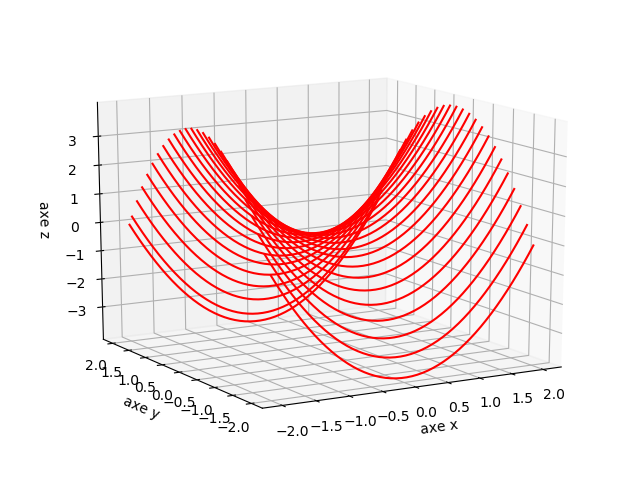
\includegraphics[scale=\myscale,scale=0.5]{figures/fonctions-quadra-3c}
		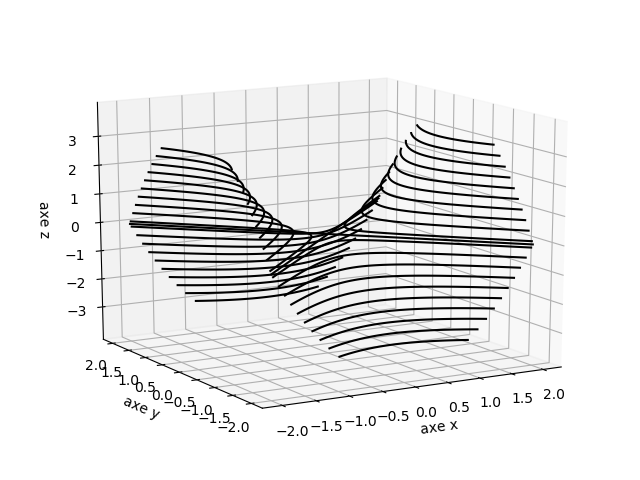
\includegraphics[scale=\myscale,scale=0.5]{figures/fonctions-quadra-3d}
		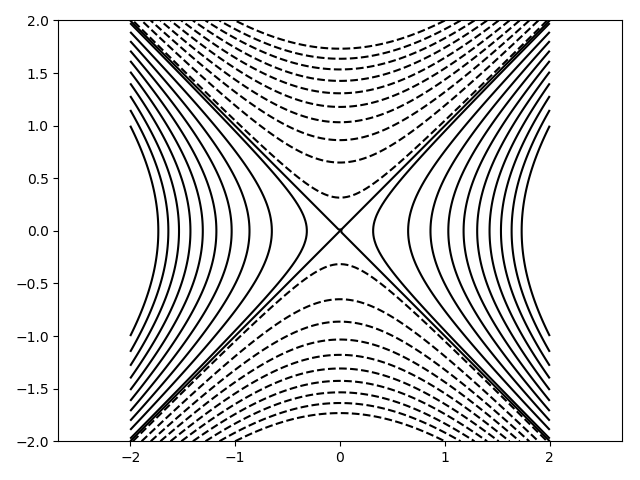
\includegraphics[scale=\myscale,scale=0.5]{figures/fonctions-quadra-3e}
	\end{center}
	
	% dessins 3d voir 'fonctions-quadra-3.py' 
\end{exemple}


%--------------------------------------------------------------------
\subsection{Régression linéaire}

\index{regression lineaire@régression linéaire}

\begin{exemple}{}{}
	On se donne des points du plan, comme ci-dessous. On s'aperçoit qu'ils sont à peu près alignés et on souhaite trouver l'équation d'une droite :
	$$y= a x + b$$ 
	qui les approche au mieux.
	
	
	\myfigure{0.6}{
		\tikzinput{fig-fonctions-10}
	}
	
	
	Formalisons un peu le problème : on se donne $N$ points $A_i(x_i,y_i)$, $i=1,\ldots,N$. Pour une droite $\mathcal{D}$ d'équation $y=ax+b$, la distance entre $A_i$ et la droite $\mathcal{D}$ est donnée par la formule :
	$$d(A_i,\mathcal{D}) = \frac{|ax_i-y_i+b|}{\sqrt{1+a^2}}.$$
	Pour se débarrasser des valeurs absolues et des racines carrées, on élève au carré et on décide que la droite qui approche au mieux tous les points $A_i$ est la droite qui minimise la fonction 
	$$f(a,b) = \sum_{i=1}^{N} d(A_i,\mathcal{D})^2 = 
	\frac{1}{1+a^2} \sum_{i=1}^{N}  (ax_i-y_i+b)^2.$$
	
	Pour les $5$ points du dessin initial : $A_1(2,3)$, $A_2(3,5)$, 
	$A_2(4,4)$, $A_4(5,6)$ et $A_5(6,6)$, il s'agit donc de trouver $(a,b)$ qui minimise la fonction 
	$$f(a,b) = \frac{1}{1+a^2} \left( 
	(2a-3+b)^2 + (3a-5+b)^2 + (4a-4+b)^2 + (5a-6+b)^2 + (6a-6+b)^2 \right).$$
	
	
	On trace le graphe de $f$, les lignes de niveau de $f$, et on utilise les techniques à notre disposition pour trouver qu'un minimum global est réalisé en $(a,b) \simeq (0.8,1.6)$, ce qui permet de tracer une droite $y=ax+b$ solution.
	
	\myfigure{0.6}{
		\tikzinput{fig-fonctions-11}
	} 
	
	Lorsque l'on dessine les lignes de niveau, on s'aperçoit que le minimum \couleurnb{(le point bleu) }{}se trouve dans une région plate et allongée. Cela signifie que, bien que le minimum $(a_{\min},b_{\min})$ soit unique, il existe beaucoup de $(a,b)$ tels que $f(a,b)$ soit proche de la valeur minimale $f(a_{\min},b_{\min})$. De plus, ces points $(a,b)$ peuvent être assez éloignés de la solution $(a_{\min},b_{\min})$ (par exemple tous les points de la zone ovale autour du \couleurnb{point bleu}{minimum}). Ce qui signifie que beaucoup de droites très différentes approchent la solution optimale.
	
	
	\begin{center}
		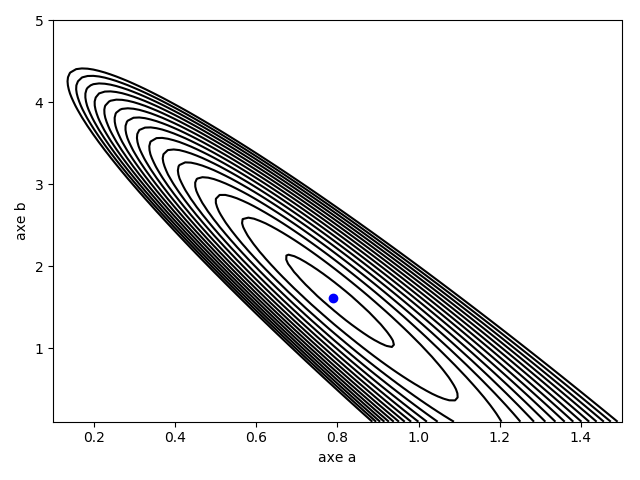
\includegraphics[scale=\myscale,scale=0.7]{figures/fonctions-regression}
	\end{center}
	% voir 'fonctions-regression-1.py'
	
\end{exemple}

%\objectifs{}



%%%%%%%%%%%%%%%%%%%%%%%%%%%%%%%%%%%%%%%%%%%%%%%%%%%%%
\section{Dérivées partielles}

Pour une fonction de plusieurs variables, il existe une dérivée pour chacune des variables, qu'on appelle dérivée partielle. 

%----------------------------------------------------
\subsection{Définition}


\begin{definition}{}{}
	Soit $f : \Rr^2 \to \Rr$. 
	La \trouer{dérivée partielle}\index{derivee partielle@dérivée partielle} $\frac{\partial f}{\partial x} (x_0,y_0)$ de $f$ par rapport à la variable $x$ au point $(x_0,y_0) \in \Rr^2$ est la dérivée en $x_0$ de 
	la fonction d'une variable $x \mapsto f(x, y_0)$.
	
	De même $\frac{\partial f}{\partial y} (x_0,y_0)$ est la dérivée partielle de $f$ par rapport à la variable $y$ au point $(x_0,y_0)$.
	
	
\end{definition}

Comme d'habitude et sauf mention contraire, nous supposerons que toutes les dérivées partielles existent.

Autrement dit, en revenant à la définition de la dérivée comme une limite :
$$\frac{\partial f}{\partial x} (x_0,y_0) = \lim_{h \rightarrow 0} 
\frac{f(x_0+h, y_0) - f(x_0,y_0)}{h}
\quad \text{ et } \quad 
\frac{\partial f}{\partial y} (x_0,y_0) = \lim_{h \rightarrow 0} 
\frac{f(x_0, y_0+h) - f(x_0,y_0)}{h}.$$




Plus généralement, pour une fonction $f : \Rr^n \to \Rr$ de plusieurs variables,
$\frac{\partial f}{\partial x_i} (x_1,\ldots,x_n)$ est la dérivée partielle de $f$ par rapport à la variable $x_i$ au point $(x_1,\ldots,x_n) \in \Rr^n$.
C'est la dérivée en $x_i$ de la fonction d'une variable $x_i \mapsto f(x_1,\ldots,x_n)$ où l'on considère fixes les variables $x_j$ pour $j \neq i$.

\bigskip

\textbf{Notations.}
$$\frac{\partial f}{\partial x} (x,y) \quad \text{ et } \quad \frac{\partial f}{\partial y} (x,y)$$
sont les analogues de l'écriture $\frac{\dd f}{\dd x}(x)$ pour l'écriture de la dérivée lorsqu'il n'y a qu'une seule variable.
Le symbole \og{}$\partial$\fg{} se lit \og{}d rond\fg{}.
Une autre notation est $\partial_x f(x,y)$, $\partial_y f(x,y)$ ou bien encore $f'_x (x,y)$, $f'_y (x,y)$.








%----------------------------------------------------
\subsection{Calculs}

La calcul d'une dérivée partielle n'est pas plus compliqué que le calcul d'une dérivée.

\textbf{Méthode.}
Pour calculer une dérivée partielle par rapport à une variable, il suffit de dériver par rapport à cette variable en considérant les autres variables comme des constantes.


\begin{exemple}{}{}
	Calculer les dérivées partielles de la fonction 
	$f : \Rr^2 \to \Rr$ définie par $f(x,y)=x^2e^{3y}$.
	
	\medskip
	\emph{Solution.}
	
	Pour calculer la dérivée partielle $\frac{\partial f}{\partial x}$, par rapport à $x$, on considère que $y$ est une constante et on dérive $x^2e ^{3y}$ comme si c'était une fonction de la variable $x$ uniquement :
	$$\frac{\partial f}{\partial x}(x,y) =2xe ^{3y}.$$
	Pour l'autre dérivée  $\frac{\partial f}{\partial y}$, on considère que $x$ est une constante et on dérive $x^2e ^{3y}$ comme si c'était une fonction de $y$ :
	$$\frac{\partial f}{\partial y}(x,y) = 3x^2e ^{3y}.$$
\end{exemple}



\begin{exemple}{}{}
	Pour $f : \Rr^3 \to \Rr$ définie par $f(x,y,z)=\cos (x+y^2)e^{-z}$ on a :
	\begin{align*}
		\frac{\partial f}{\partial x}(x,y,z) = -\sin(x+y^2)e^{-z}, \\
		\frac{\partial f}{\partial y}(x,y,z) = -2y\sin(x+y^2)e^{-z}, \\
		\frac{\partial f}{\partial z}(x,y,z) = -\cos(x+y^2)e^{-z}.
	\end{align*}
\end{exemple}


\begin{exemple}{}{}
	Soit $f :\Rr^n \to \Rr$ définie par 
	$f(x_1,\ldots,x_n) = x_1^2+x_2^2+\cdots + x_n^2$,
	alors pour $i=1,\ldots,n$ :
	$$\frac{\partial f}{\partial x_i}(x_1,\ldots,x_n) = 2x_i.$$
\end{exemple}


%----------------------------------------------------
\subsection{Interprétation géométrique}


Pour une fonction d'une variable, la dérivée est la pente de la tangente au graphe de la fonction (le graphe étant alors une courbe). Pour une fonction de deux variables $(x,y) \mapsto f(x,y)$, les dérivées partielles indiquent les pentes au graphe de $f$ selon certaines directions (le graphe étant ici une surface). Plus précisément :

\begin{itemize}
	\item $\frac{\partial f}{\partial x} (x_0,y_0)$ est la pente du graphe de $f$
	en $(x_0,y_0)$ suivant la direction de l'axe $(Ox)$.
	En effet cette pente est celle de la tangente à la courbe $z = f(x,y_0)$ et est donnée par la dérivée de $x \mapsto f(x,y_0)$ en $x_0$, c'est donc bien $\frac{\partial f}{\partial x} (x_0,y_0)$.
	
	\item $\frac{\partial f}{\partial y} (x_0,y_0)$ est la pente du graphe de $f$
	en $(x_0,y_0)$ suivant la direction de l'axe $(Oy)$.
	
	
\end{itemize}



\bigskip 
Sur la figure de gauche, la dérivée partielle  $\frac{\partial f}{\partial x}$ indique la pente de la tranche parallèle à l'axe $(Ox)$\couleurnb{ (en orange)}{}. Sur la figure de droite, la dérivée partielle  $\frac{\partial f}{\partial y}$ indique la pente de la tranche parallèle à l'axe $(Oy)$\couleurnb{ (en vert)}{}.


\myfigure{0.75}{
	\tikzinput{fig-calculdiff-04}
	\tikzinput{fig-calculdiff-05}
} 





%%%%%%%%%%%%%%%%%%%%%%%%%%%%%%%%%%%%%%%%%%%%%%%%%%%%%
\section{Gradient}

Le gradient est un vecteur dont les coordonnées sont les dérivées partielles. Il a de nombreuses applications géométriques car il donne l'équation des tangences aux courbes et surfaces de niveau. Surtout, il indique la direction dans laquelle la fonction varie le plus vite.

Le gradient est un vecteur qui remplace la notion de dérivée pour les fonctions de plusieurs variables. On sait que la dérivée permet de décider si une fonction est croissante ou décroissante. De même, le vecteur gradient indique la direction dans laquelle la fonction croît ou décroît le plus vite. Nous allons voir comment calculer de façon algorithmique le gradient grâce à la \og{}différentiation automatique\fg{}.

%----------------------------------------------------
\subsection{Définition}

\begin{definition}{}{}
	Soit $f : \Rr^2 \to \Rr$ une fonction admettant des dérivées partielles.
	Le \trouer{gradient}\index{gradient} de $f$ en $(x_0,y_0) \in \Rr^2$, noté 
	$\grad f (x_0,y_0)$, est le vecteur :
	$$\grad f (x_0,y_0) =
	\begin{pmatrix} \dfrac{\partial f}{\partial x} (x_0,y_0)\\[2ex] \dfrac{\partial f}{\partial y}(x_0,y_0)\end{pmatrix}.$$
\end{definition}

Les physiciens et les anglo-saxons notent souvent $\nabla f (x,y)$ pour $\grad f (x,y)$. Le symbole $\nabla$ se lit \og{}nabla\fg{}.


Plus généralement, pour $f : \Rr^n \to \Rr$, le gradient de $f$ en $(x_1,\ldots,x_n) \in \Rr^n$ est le vecteur :
$$\grad f (x_1,\ldots,x_n) =
\begin{pmatrix} \dfrac{\partial f}{\partial x_{1}} (x_1,\ldots,x_n)\\ \vdots \\ \dfrac{\partial f}{\partial x_n}(x_1,\ldots,x_n)\end{pmatrix}.$$



\begin{exemple}{}{}
	\begin{itemize}
		\item $f(x,y) = x^2y^3$, $\grad f (x,y) =  \begin{pmatrix}2xy^3\\3x^2y^2\end{pmatrix}$. Au point $(x_0,y_0)=(2,1)$, $\grad f (2,1) =  \begin{pmatrix}4\\12\end{pmatrix}$.
		
		\item $f(x,y,z) = x^2\sin(yz)$, $\grad f (x,y,z) = \begin{pmatrix} 2x\sin(yz) \\ x^2z \cos(yz) \\ x^2y\cos(yz) \end{pmatrix}$.
		
		\item $f(x_1,\ldots,x_n)= x_1^2+x_2^2+\cdots + x_n^2$, $\grad f (x_1,\ldots,x_n) =  \begin{pmatrix}2x_1\\ \vdots \\2x_n\end{pmatrix}$.
	\end{itemize}
\end{exemple}



%----------------------------------------------------
\subsection{Tangentes aux lignes de niveau}


Soit $f : \Rr^2 \to \Rr$ une fonction différentiable. On considère les lignes de niveau $f(x,y)=k$.


\begin{proposition}{}{}
	\index{lignes de niveau}
	Le vecteur gradient $\grad f(x_0,y_0)$ est orthogonal à la ligne de niveau de $f$ passant au point $(x_0,y_0)$. 
\end{proposition}


Sur ce premier dessin, sont dessinés la ligne de niveau passant par le point $(x_0,y_0)$ \couleurnb{(en rouge)}{}, un vecteur tangent $v$ en ce point et la tangente à la ligne de niveau\couleurnb{ (en vert)}{}. 
Le vecteur gradient est un vecteur du plan qui est orthogonal à la ligne de niveau en ce point\couleurnb{ (en bleu)}{}.


\bigskip

\myfigure{0.8}{
	\tikzinput{fig-gradient-02}
}

À chaque point du plan, on peut associer un vecteur gradient. Ce vecteur gradient est orthogonal à la ligne de niveau passant par ce point. Nous verrons juste après comment savoir s'il est orienté \og{}vers le haut\fg{} ou \og{}vers le bas\fg{}. 

\myfigure{0.8}{
	\tikzinput{fig-gradient-01}
}

Dans le cadre de notre étude, nous nous intéressons à l'équation de la tangente.
\begin{proposition}{}{}
	\index{tangente}
	Au point $(x_0,y_0)$, l'équation de la tangente à la ligne de niveau de $f$ est :
	$$\frac{\partial f}{\partial x}(x_0,y_0)(x-x_0)+\frac{\partial f}{\partial y}(x_0,y_0)(y-y_0)=0$$
	pourvu que le gradient de $f$ en ce point ne soit pas le vecteur nul.
\end{proposition}



\begin{exemple}{Tangentes à une ellipse}{}
	Trouver les tangentes à l'ellipse $\mathcal{E}$ d'équation $\frac{x^2}{a^2}+\frac{y^2}{b^2} = 1$.
	
	\myfigure{0.7}{
		\tikzinput{fig-gradient-03}
	}
	
	Cette ellipse $\mathcal{E}$ est la ligne de niveau $f(x,y)=1$ de la fonction
	$f(x,y) = \frac{x^2}{a^2}+\frac{y^2}{b^2}$. 
	Les dérivées partielles en $(x_0, y_0)$ sont :
	$$\frac{\partial f}{\partial x}(x_0,y_0) = \frac{2x_0}{a^2} \qquad \text{ et } \qquad \frac{\partial f}{\partial y}(x_0,y_0) = \frac{2y_0}{b^2}.$$
	L'équation de la tangente à l'ellipse $\mathcal{E}$ en ce point est donc :
	$$\frac{2x_0}{a^2}(x-x_0)+\frac{2y_0}{b^2}(y-y_0)=0.$$
	Mais comme $\frac{x_0^2}{a^2}+\frac{y_0^2}{b^2} = 1$, l'équation de la tangente se simplifie en $\displaystyle \frac{x_0}{a^2}x + \frac{y_0}{b^2} y = 1$.
\end{exemple}


%----------------------------------------------------
\subsection{Lignes de plus forte pente}

Considérons les lignes de niveau $f(x,y)=k$ d'une fonction $f : \Rr^2 \to \Rr$.
On se place en un point $(x_0,y_0)$. On cherche dans quelle direction se déplacer pour augmenter au plus vite la valeur de $f$.

\begin{proposition}{}{}
	Le vecteur gradient $\grad f(x_0,y_0)$ indique la direction de plus grande pente à partir du point $(x_0,y_0)$.
\end{proposition}


Autrement dit, si l'on veut, à partir d'un point donné $(x_0,y_0)$ de niveau $a$, passer au niveau $b>a$ le plus vite possible alors il faut démarrer en suivant la direction du gradient $\grad f(x_0,y_0)$. 

\myfigure{1}{
	\tikzinput{fig-gradient-05}
}

Comme illustration, un skieur de descente, voulant optimiser sa course, choisira en permanence de s'orienter suivant la plus forte pente, c'est-à-dire dans le sens opposé au gradient. 

%----------------------------------------------------
\subsection{Dérivée directionnelle}

Pour prouver que le gradient indique la ligne de la plus grande pente, nous avons besoin de généraliser la notion de dérivée partielle. Ce passage est plus technique et peut être ignoré en première lecture.

Soit $v=\left(\begin{smallmatrix}h\\k\end{smallmatrix}\right)$ un vecteur du plan.
La \trouer{dérivée directionnelle} de $f$ suivant le vecteur $v$ en $(x_0,y_0)$ est le nombre :
$$D_v f(x_0,y_0) = h\frac{\partial f}{\partial x}(x_0,y_0)
+k\frac{\partial f}{\partial y}(x_0,y_0).$$


La dérivée directionnelle correspond à la pente de la fonction pour la tranche dirigée par le vecteur $v$.

\myfigure{0.8}{
	\tikzinput{fig-calculdiff-06}
} 

Remarque : pour $v=\left(\begin{smallmatrix}1\\0\end{smallmatrix}\right)$
alors $D_v f(x_0,y_0) = \frac{\partial f}{\partial x}(x_0,y_0)$ et pour 
$v=\left(\begin{smallmatrix}0\\1\end{smallmatrix}\right)$
alors $D_v f(x_0,y_0) = \frac{\partial f}{\partial y}(x_0,y_0)$.


On rappelle que le \trouer{produit scalaire} de deux vecteurs $u=\left(\begin{smallmatrix}x\\y\end{smallmatrix}\right)$ et 
$v=\left(\begin{smallmatrix}x'\\y'\end{smallmatrix}\right)$
est donné par 
$$\langle u \mid v \rangle = xx' + yy'.$$
On sait que le produit scalaire se calcule aussi géométriquement par :
$$\langle u \mid v \rangle = \|u\|\cdot \|v\| \cdot \cos(\theta)$$
où $\theta$ est l'angle entre $u$ et $v$.

\myfigure{1}{
	\tikzinput{fig-scalaire}
} 


Ainsi, on peut réécrire la dérivée directionnelle sous la forme :
$$D_v f(x_0,y_0) = \langle \grad f (x_0,y_0) \mid v \rangle.$$


On peut maintenant prouver que le gradient indique la ligne de plus grande pente.

\begin{proof}
	La dérivée suivant le vecteur non nul $v$ au point $(x_0,y_0)$ décrit la variation de $f$ autour de ce point lorsqu'on se déplace dans la direction $v$. 
	La direction selon laquelle la croissance est la plus grande est celle du gradient de $f$. En effet,
	$$D_{v}f(x_0,y_0)=\langle \grad f(x_0,y_0) \mid v\rangle=
	\| \grad f(x_0,y_0) \| \cdot \| v \| \cdot \cos \theta$$
	où $\theta$ est l'angle entre le vecteur $\grad f(x_0,y_0)$ et le vecteur $v$.
	Le maximum est atteint lorsque l'angle $\theta=0$, c'est-à-dire lorsque $v$ pointe dans la même direction que $\grad f(x_0,y_0)$.
\end{proof}


%----------------------------------------------------
\subsection{Surface de niveau}

Les résultats présentés ci-dessus pour les fonctions de deux variables se généralisent aux fonctions de trois variables ou plus.
Commençons avec trois variables et une fonction $f:\Rr^3 \to \Rr$.
Rappelons qu'un plan de $\Rr^3$ passant par $(x_0,y_0,z_0)$ et de vecteur normal 
$n=(a,b,c)$ a pour équation cartésienne :
$$a(x-x_0)+b(y-y_0)+c(z-z_0) = 0.$$


De même qu'il existe une droite tangente pour les lignes de niveau, il existe un \trouer{plan tangent} à une surface de niveau.


\begin{proposition}{}{}
	Le vecteur gradient $\grad f(x_0,y_0,z_0)$ est orthogonal à la surface de niveau de $f$ passant au point $(x_0,y_0,z_0)$. Autrement dit,
	l'équation du plan tangent à la surface de niveau de $f$ en $(x_0,y_0,z_0)$ est 
	$$\frac{\partial f}{\partial x}(x_0,y_0,z_0)(x-x_0)
	+\frac{\partial f}{\partial y}(x_0,y_0,z_0)(y-y_0)
	+\frac{\partial f}{\partial z}(x_0,y_0,z_0)(z-z_0)
	= 0 $$
	pourvu que le gradient de $f$ en ce point ne soit pas le vecteur nul.
\end{proposition}


\myfigure{1}{
	\tikzinput{fig-gradient-07}
}


Plus généralement pour $f : \Rr^n \to \Rr$, $\grad f (x_1,\ldots,x_n)$ est orthogonal à l'espace tangent à
l'hypersurface de niveau $f=k$ passant par le point $(x_1,\ldots,x_n)\in\Rr^n$ et 
ce vecteur gradient $\grad f(x_1,\ldots,x_n)$ indique la direction de plus grande pente à partir du point $(x_1,\ldots,x_n)$.



%----------------------------------------------------
\subsection{Calcul approché}

Rappelez-vous que la dérivée nous a permis de faire des calculs approchés, par exemple pour estimer $\sqrt{1.01}$ sans calculatrice (voir le chapitre \og{}Dérivée\fg{}).
Voici, en deux variables, l'analogue de la formule pour une variable : 
$$f(x_0+h,y_0+k) \simeq f(x_0,y_0) + h\frac{\partial f}{\partial x}(x_0,y_0)
+k\frac{\partial f}{\partial y}(x_0,y_0).$$
Cette approximation est valable pour $h$ et $k$ petits.

L'interprétation géométrique est la suivante : 
on approche le graphe de $f$ en $(x_0,y_0)$ par le plan tangent au graphe en ce point. Sur la figure ci-dessous sont représentés : le graphe de $f$\couleurnb{ (en rouge)}{}, le plan tangent au-dessus du point $(x_0,y_0)$\couleurnb{ (en bleu)}{}. La valeur $z_1 = f(x_0+h,y_0+k)$ est la valeur exacte donnée par le point de la surface au dessus de $(x_0+h,y_0+k)$. On approche cette valeur par $z_2 = f(x_0,y_0) + h\frac{\partial f}{\partial x}(x_0,y_0)
+k\frac{\partial f}{\partial y}(x_0,y_0)$ donnée par le point du plan tangent au dessus de $(x_0+h,y_0+k)$. 


\myfigure{1}{
	\tikzinput{fig-gradient-10}
}


\begin{exemple}{}{}
	Valeur approchée de $f(1.002, 0.997)$ si $f(x,y) = x^2y$.
	\bigskip
	
	\emph{Solution.}
	Ici $(x_0,y_0) = (1,1)$, $h = 2 \times 10^{-3}$, $k = -3 \times 10^{-3}$,
	$\frac{\partial f}{\partial x}(x,y) = 2xy$, $\frac{\partial f}{\partial y}(x,y) = x^2$, donc $\frac{\partial f}{\partial x}(x_0,y_0) = 2$, $\frac{\partial f}{\partial y}(x_0,y_0) = 1$. Ainsi
	$$f(1+h,1+k) \simeq f(1,1) + 2h + k$$
	donc 
	$$f(1.002, 0.997) \simeq 1 + 2 \times 2 \times 10^{-3} - 3 \times 10^{-3} \simeq 1.001.$$
	Avec une calculatrice, on trouve $f(1.002, 0.997) = 1.000992$ : l'approximation est bonne.
\end{exemple}


%----------------------------------------------------
\subsection{Minimum et maximum}

\begin{definition}{}{}
	\index{minimum!local}
	Soit $f : \Rr^2 \to \Rr$.
	\begin{itemize}
		\item La fonction $f$ admet un \trouer{minimum local} en $(x_0,y_0)$ s'il existe un disque $D$ centré en ce point tel que 
		$$ f(x,y) \ge f(x_0,y_0) \quad \text{ pour tout } (x,y) \in D.$$
		\item La fonction $f$ admet un \trouer{maximum local} en $(x_0,y_0)$  pour lequel 
		$$f(x,y) \le f(x_0,y_0) \quad \text{ pour tout } (x,y) \in D.$$
		\item On parle d'un \trouer{extremum local} pour un minimum ou un maximum local.
	\end{itemize}
\end{definition}

% [[dessins 3D min/max]]

\begin{exemple}{}{}
	L'exemple type de minimum est celui de la fonction $f(x,y)=x^2+y^2$ en $(0,0)$.
	Voici son graphe et ses lignes de niveau.
	
	\begin{center}
		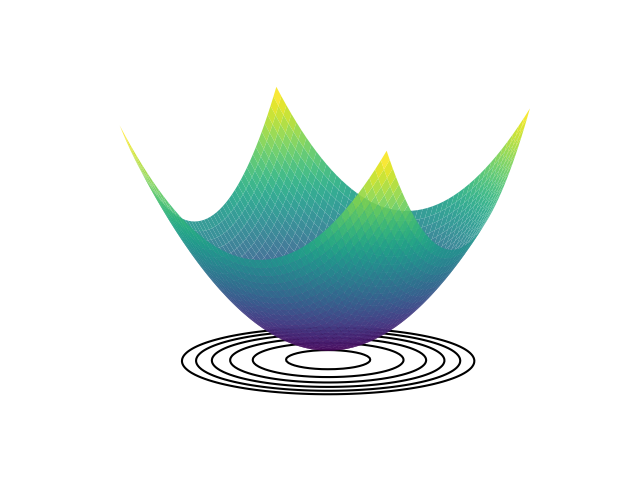
\includegraphics[scale=\myscale,scale=0.7]{figures/gradient-surface-1a}
	\end{center}
	
	
	La fonction $f(x,y) = -x^2-y^2$ admet, elle, un maximum en $(0,0)$.
	\begin{center}
		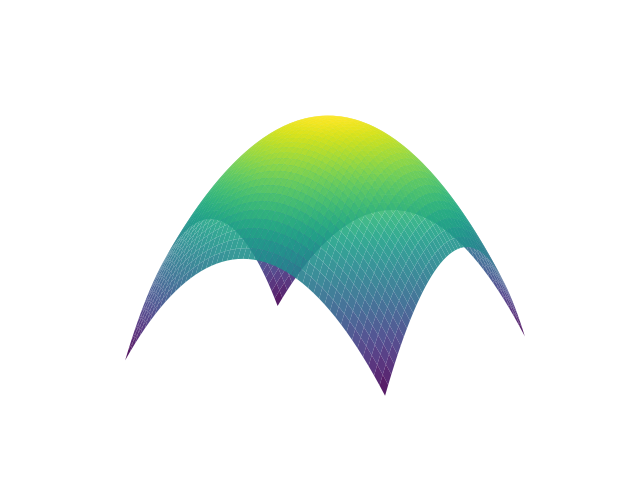
\includegraphics[scale=\myscale,scale=0.7]{figures/gradient-surface-2}
	\end{center}
	
\end{exemple}

\begin{proposition}{}{}
	Soit $f : \Rr^2 \to \Rr$. Si $f$ admet un minimum ou un maximum local en $(x_0,y_0)$ alors le gradient est le vecteur nul en ce point, autrement dit :
	$$
	\frac{\partial f}{\partial x}(x_0,y_0) = 0 
	\quad \text{ et  }\quad
	\frac{\partial f}{\partial y}(x_0,y_0) = 0.
	$$
\end{proposition}

\begin{proof}
	Prenons le cas d'un minimum local.
	La fonction d'une variable $x \mapsto f(x, y_0)$ admet aussi un minimum en $x_0$ donc sa dérivée est nulle en $x_0$, c'est-à-dire $\frac{\partial f}{\partial x}(x_0,y_0) = 0$. De même $y \mapsto f(x_0, y)$ admet un minimum en $y_0$ donc $\frac{\partial f}{\partial y}(x_0,y_0) = 0$. 
\end{proof}


Dans la suite du cours nous chercherons les points pour lesquels une fonction donnée présente un minimum local.
D'après la proposition précédente, ces points sont à chercher parmi les points en lesquels le gradient s'annule. On dira que $(x_0,y_0)$ est un \trouer{point critique}\index{point critique} de $f$ si
les deux dérivées partielles $\frac{\partial f}{\partial x}(x_0,y_0)$ et $\frac{\partial f}{\partial y}(x_0,y_0)$ s'annulent simultanément.

\begin{exemple}{}{}
	Chercher les points en lesquels $f(x,y) = x^2-y^3+xy$ peut atteindre son minimum.
	
	\textbf{Recherche des points critiques.}
	On calcule 
	$$\frac{\partial f}{\partial x}(x,y) = 2x+y 
	\quad \text{ et } \quad 
	\frac{\partial f}{\partial y}(x,y) = -3y^2+x.$$
	On cherche les points $(x,y)$ en lesquels les deux dérivées partielles s'annulent.
	Par l'annulation de la première dérivée, on a $2x+y=0$ donc $y=-2x$.
	Par l'annulation de la seconde dérivée, on a $-3y^2+x=0$ ce qui donne par substitution
	$-12x^2+x=0$, ainsi $x(-12x+1)=0$.
	Donc soit $x=0$ et alors on a $y=0$, soit $x=\frac1{12}$ et alors $y=-\frac16$.
	Bilan : il y a deux points critiques :
	$$\left(0,0\right) \quad \text{ et } \quad \left(\frac1{12},-\frac16\right).$$
	
	\textbf{\'Etude du point critique $(0,0)$.}
	On a $f(0,0)=0$ mais on remarque que $f(0,y)=-y^3$ qui peut être négatif ou positif (selon le signe de $y$ proche de $0$), donc en $(0,0)$ il n'y a ni minimum ni maximum.
	
	\textbf{\'Etude du point critique $(\frac1{12},-\frac16)$.}
	Il existe un critère (que l'on ne décrira pas ici) qui permet de dire qu'en ce point $f$ admet un minimum local.
	
	Sur le dessin ci-dessous, le minimum est situé à l'intérieur du petit ovale, l'autre point critique en $(0,0)$ correspond à l'intersection de la ligne de niveau $f=0$ avec elle-même.
	\begin{center}
		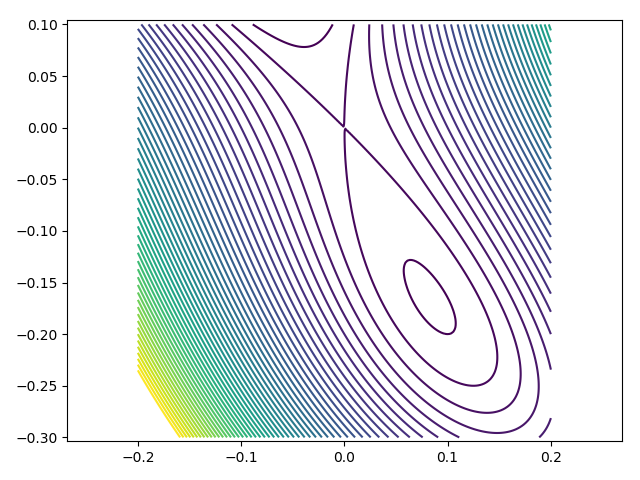
\includegraphics[scale=\myscale,scale=0.7]{figures/gradient-surface-6}
	\end{center}
	
\end{exemple}
Sur l'exemple précédent, nous avons assez facilement calculé les points critiques à partir des deux équations à deux inconnues. Il faut prendre garde que ce n'est pas un système linéaire et que dans le cas d'une fonction plus compliquée il aurait été impossible de déterminer exactement les points critiques.

On note aussi dans l'exemple précédent que certains points critiques ne sont ni des maximums ni des minimums. L'exemple type, illustré ci-dessous, est celui d'un \trouer{col} appelé aussi \trouer{point-selle}\index{point-selle} en référence à sa forme de selle de cheval.

\begin{exemple}{}{}
	Soit $f(x,y)=x^2-y^2$.
	Voici son graphe vu sous trois angles différents et ses lignes de niveau.
	
	\begin{center}
		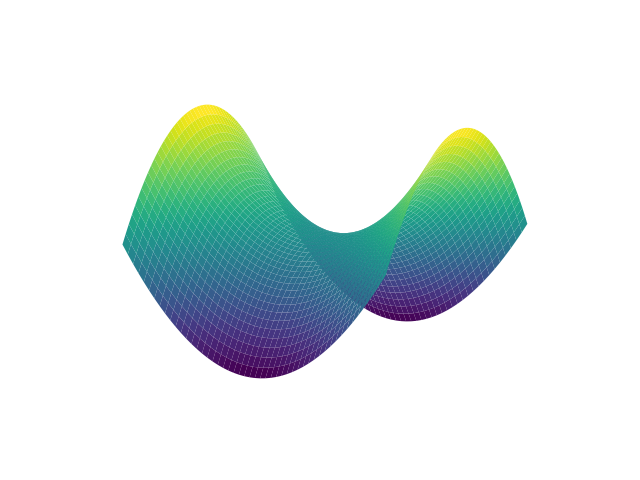
\includegraphics[scale=\myscale,scale=0.7]{figures/gradient-surface-3a}
	\end{center}
	\begin{center}
		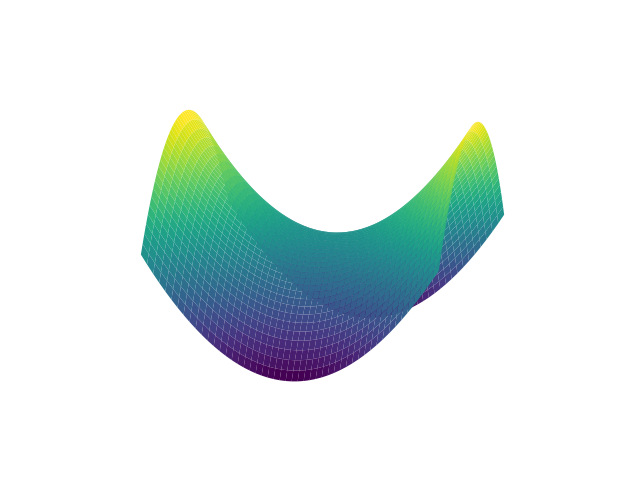
\includegraphics[scale=\myscale,scale=0.5]{figures/gradient-surface-3b}
		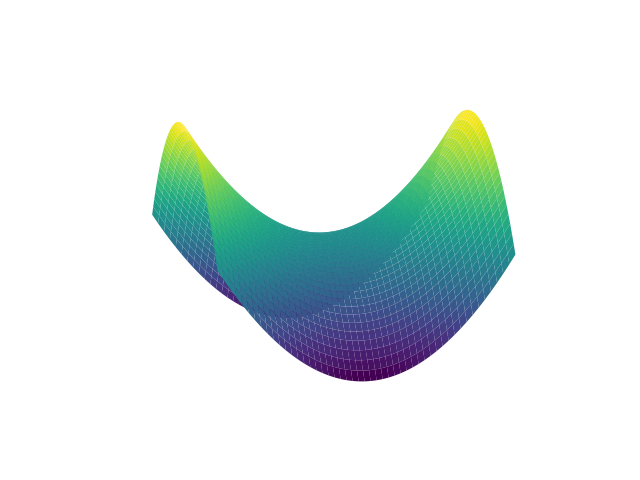
\includegraphics[scale=\myscale,scale=0.5]{figures/gradient-surface-3c}
	\end{center}
	\begin{center}
		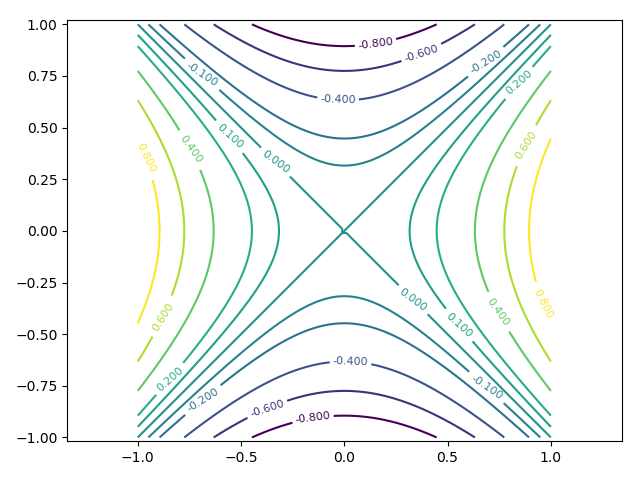
\includegraphics[scale=\myscale,scale=0.7]{figures/gradient-surface-4}
	\end{center}
	
	
\end{exemple}


Comme il peut être difficile de calculer les points critiques de façon exacte, nous allons utiliser des méthodes numériques.
L'idée qui sera détaillée dans le prochain chapitre est la suivante : comme le gradient indique la direction dans laquelle la fonction $f$ croît le plus rapidement, nous allons suivre la direction opposée au gradient, pour laquelle $f$ décroît le plus rapidement. Ainsi, partant d'un point $(x_0,y_0)$ au hasard, on sait dans quelle direction se déplacer pour obtenir un nouveau point $(x_1,y_1)$ en lequel $f$ est plus petite. Et on recommence.

Sur les trois dessins ci-dessous, on a dessiné les lignes de niveau d'une fonction $f$ ainsi que les vecteurs $-\grad f(x,y)$. On voit que ces vecteurs pointent bien vers le minimum (figure de gauche), s'éloignent d'un maximum (figure centrale), le cas d'un point-selle est spécial (figure de droite). Dans tous les cas, la longueur des vecteurs gradients diminue à l'approche du point critique.


\begin{center}
	\begin{minipage}{0.30\textwidth}
		\center
		\ \ 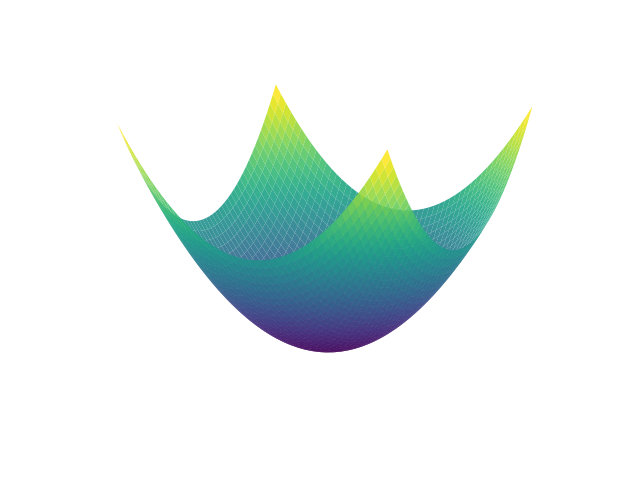
\includegraphics[scale=\myscale,scale=0.35]{figures/gradient-surface-1b}\\
		
		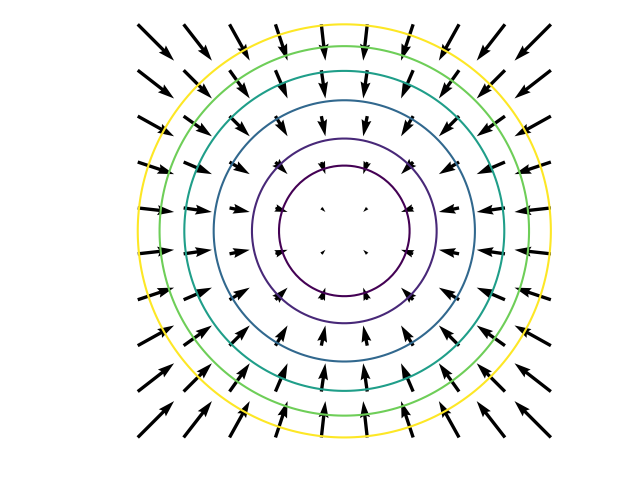
\includegraphics[scale=\myscale,scale=0.35]{figures/gradient-surface-5a}
		
		\quad\textbf{Cas d'un minimum}
	\end{minipage}
	\begin{minipage}{0.30\textwidth}
		\center
		
		\ \ 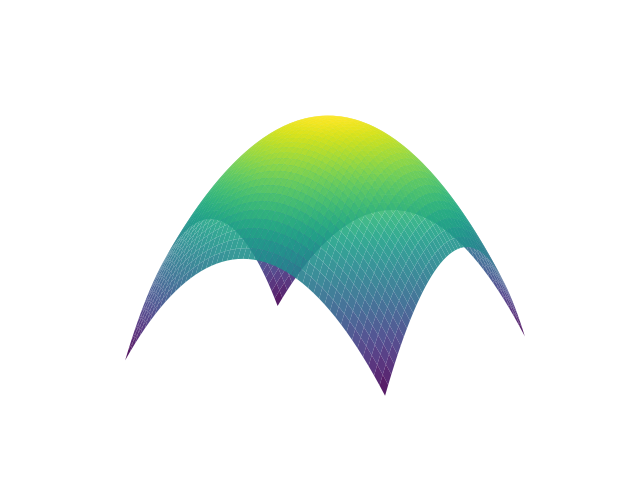
\includegraphics[scale=\myscale,scale=0.35]{figures/gradient-surface-2}\\
		
		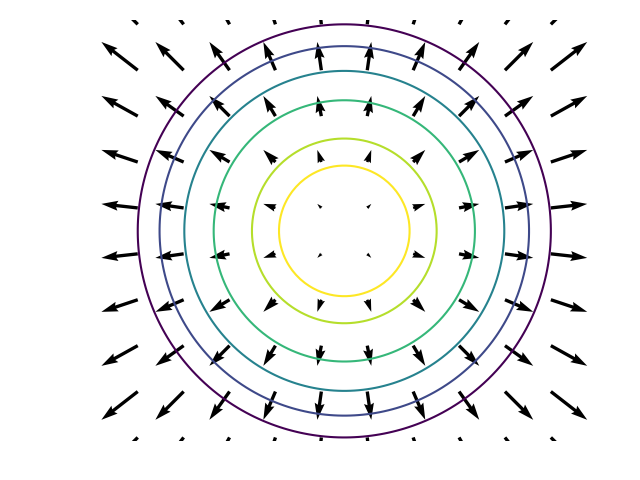
\includegraphics[scale=\myscale,scale=0.35]{figures/gradient-surface-5b}
		
		\quad\textbf{Cas d'un maximum}
	\end{minipage}
	\begin{minipage}{0.30\textwidth}
		\center
		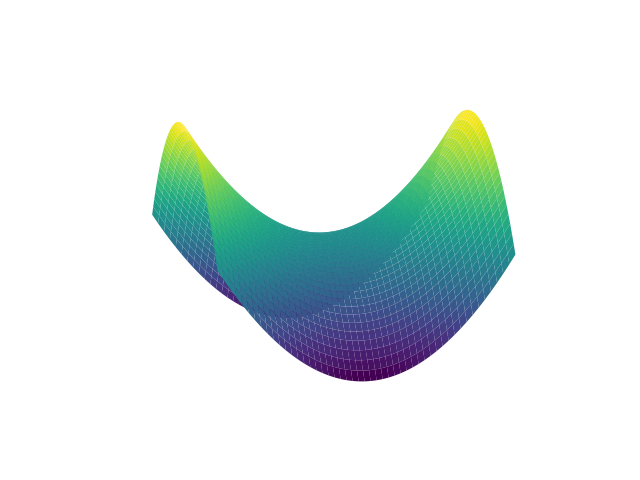
\includegraphics[scale=\myscale,scale=0.35]{figures/gradient-surface-3c}\\
		
		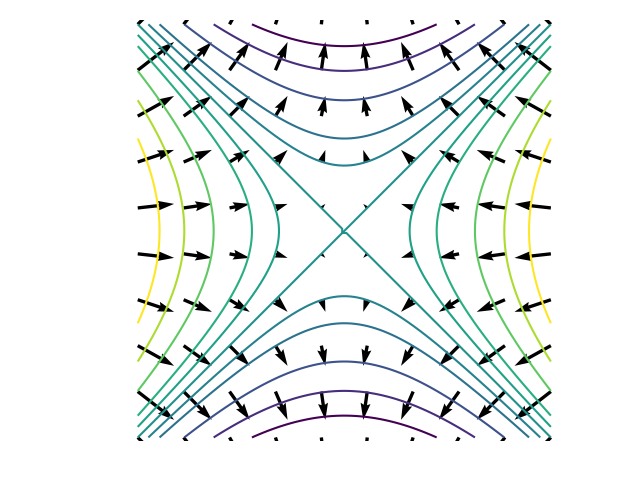
\includegraphics[scale=\myscale,scale=0.35]{figures/gradient-surface-5c}
		
		\quad\textbf{Cas d'un point-selle}
	\end{minipage}
\end{center}

%%%%%%%%%%%%%%%%%%%%%%%%%%%%%%%%%%%%%%%%%%%%%%%%%%%%%%%%%%%%%%%%%%%%%
\section{Différentiation automatique}

\index{différentiation automatique}

Dans le chapitre \og{}Dérivée\fg{}, nous avons vu comment calculer la dérivée d'une fonction composée à l'aide de son graphe de calcul. Nous allons faire de même pour les dérivées partielles des fonctions de plusieurs variables afin de calculer le gradient d'une fonction définie par un réseau de neurones.

%--------------------------------------------------------------------
\subsection{Différentiation automatique}

\textbf{Graphe de calcul.}\index{graphe de calcul}
Voici le graphe de calcul d'une fonction $f$ de deux variables (schéma de principe à gauche, évaluation en $(x_0,y_0)$ à droite).

\myfigure{0.6}{
	\tikzinput{fig-diffauto-01}\qquad\qquad\qquad
	\tikzinput{fig-diffauto-02}
}


\bigskip
\textbf{Dérivées locales.}
Voici la règle pour les dérivées locales à rajouter à chaque branche (entre crochets).
\myfigure{0.6}{
	\tikzinput{fig-diffauto-03}
}
On note $\partial_x f$ comme raccourci de la fonction $\frac{\partial f}{\partial x}$.


\bigskip
\textbf{Dérivées partielles.}
On obtient chacune des dérivées partielles d'une composition $F$ comme le produit des dérivées locales le long des branches allant de la sortie $F(x,y)$ vers l'entrée $x$ (ou $y$).
\myfigure{0.8}{
	\tikzinput{fig-diffauto-04}
}


\bigskip
\textbf{Formule mathématique.}
Soit $f : \Rr^2 \to \Rr$ et $g : \Rr \to \Rr$. 

\myfigure{0.6}{
	\tikzinput{fig-diffauto-05}
}
La composition $F = g \circ f : \Rr^2 \to \Rr$ correspond au graphe de calcul dessiné ci-dessous :
\myfigure{0.6}{
	\tikzinput{fig-diffauto-06}
}

On a donc :
$$F(x,y) = g \circ f (x,y) = g \big( f(x,y) \big).$$
Les dérivées partielles de $F$ sont données par les formules :
\mybox{$\displaystyle
	\begin{array}{c}
		\displaystyle \frac{\partial F}{\partial x}(x_0,y_0) = \frac{\partial f}{\partial x}(x_0,y_0) \cdot g'\big(f(x_0,y_0)\big)\\[4ex]
		\displaystyle \frac{\partial F}{\partial y}(x_0,y_0) = \frac{\partial f}{\partial y}(x_0,y_0) \cdot g'\big(f(x_0,y_0)\big)
	\end{array}
	$}

La preuve de la formule pour $\frac{\partial F}{\partial x}(x_0,y_0)$ découle directement de la formule de la dérivée d'une composition pour la fonction d'une seule variable $x \mapsto F(x,y_0)$. Il en est de même pour l'autre dérivée partielle.
Ces formules justifient notre règle de calcul : la dérivée partielle est le produit des dérivées locales le long de chacune des branches.

\myfigure{0.8}{
	\tikzinput{fig-diffauto-07}
}


\bigskip
\textbf{Addition et multiplication.}

Dans le cas $f(x,y) = x + y$ et $f(x,y)= x \times y$, on retrouve les dérivées locales déjà utilisées dans le cas d'une seule variable.

\myfigure{0.6}{
	\tikzinput{fig-diffauto-08}\qquad\qquad\qquad
	\tikzinput{fig-diffauto-09}
}



\bigskip
\textbf{Exemple.}
Soit $F(x,y) = \ln(x^2y+\sin y)$. On souhaite calculer $\grad F(3,2)$.
Nous allons montrer comment calculer $\grad F(x_0,y_0)$ pour $x_0$ et $y_0$ quelconques, puis nous reprendrons les calculs depuis le début dans le cas $(x_0,y_0)=(3,2)$.

\myfigure{0.8}{
	\tikzinput{fig-diffauto-10}
}
\myfigure{0.8}{
	\tikzinput{fig-diffauto-11}
}

On obtient les dérivées partielles comme produit des dérivées locales :
$$\frac{\partial F}{\partial x} (x_0,y_0) = \left[ \frac{1}{z_0} \right] \times [2x_0y_0] = \frac{2x_0y_0}{x_0^2y_0+\sin y_0},$$
$$\frac{\partial F}{\partial y} (x_0,y_0) = \left[ \frac{1}{z_0} \right] \times [x_0^2 + \cos y_0] = \frac{x_0^2 + \cos y_0}{x_0^2y_0+\sin y_0}.$$



Dans la pratique, pour les réseaux de neurones, on ne calcule jamais l'expression formelle de $\grad F(x_0,y_0)$ mais seulement des gradients en des valeurs $(x_0,y_0)$ données. On reprend donc à chaque fois les étapes ci-dessus mais uniquement pour des valeurs numériques.



La première étape est de calculer les valeurs des fonctions (de la gauche vers la droite).
\myfigure{0.8}{
	\tikzinput{fig-diffauto-12}
}

La seconde étape est de calculer toutes les dérivées locales. On utilise les valeurs de l'étape précédente et la connaissance des formules de chacune des dérivées des fonctions élémentaires (ici $\frac{\partial f}{\partial x}$, $\frac{\partial f}{\partial y}$ et $\frac{\dd \ln}{\dd z}$).

\myfigure{0.8}{
	\tikzinput{fig-diffauto-13}
}

On calcule le produit des dérivées locales le long des arêtes. 
\myfigure{0.8}{
	\tikzinput{fig-diffauto-14}
}

On obtient les dérivées partielles :
{\small
	$$\frac{\partial F}{\partial x} (3,2) = \left[ \frac{1}{18+\sin 2} \right] \times [12] = \frac{12}{18 + \sin 2}
	\qquad \text{ et } \qquad 
	\frac{\partial F}{\partial y} (3,2) = \left[ \frac{1}{18+\sin 2} \right] \times [9 + \cos 2] = \frac{9 + \cos 2}{18+\sin 2}.$$
}

\bigskip
\textbf{Règle générale.}
Dans le cas de $n$ entrées $(x_1,\ldots,x_n)$, la règle des dérivées locales se généralise naturellement : on associe à la branche numéro $i$ la dérivée locale $\frac{\partial f}{\partial x_i}$.

\myfigure{0.8}{
	\tikzinput{fig-diffauto-15}
}


%--------------------------------------------------------------------
\subsection{Différentiation automatique (suite)}


\textbf{Graphe de calcul.}
Voici le graphe de calcul d'une situation que l'on a déjà rencontrée dans le cas d'une seule variable, mais dont la formule se justifie par les fonctions de deux variables.
Il s'agit du graphe de calcul de $F(t) = f\big( u(t), v(t) \big)$ où
$u : \Rr \to \Rr$, $v : \Rr \to \Rr$ et $f : \Rr^2 \to \Rr$. L'objectif est de calculer $F'(t)$.

\myfigure{0.55}{
	\tikzinput{fig-diffauto-21}\qquad
	\tikzinput{fig-diffauto-22}
}

\bigskip
\textbf{Dérivées locales.}
On calcule les dérivées locales comme d'habitude.
\myfigure{0.8}{
	\tikzinput{fig-diffauto-23}
}

\bigskip
\textbf{Dérivée.}
La dérivée s'obtient en deux étapes :
\begin{itemize}
	\item on calcule le produit des dérivées locales le long des chemins partant de chaque arête sortante jusqu'à la sortie,
	\item puis on calcule la somme de ces produits.
\end{itemize}

\myfigure{0.9}{
	\tikzinput{fig-diffauto-24}
}

\bigskip
\textbf{Formule mathématique.}
La situation est cette fois la suivante :
\myfigure{0.6}{
	\tikzinput{fig-diffauto-25}
}
La formule de dérivation de la composition de
$$F(t) = f\big( u(t), v(t) \big)$$
est :
\mybox{$\displaystyle
	F'(t_0) = u'(t_0) \frac{\partial f}{\partial x}(u(t_0),v(t_0)) \  + \  v'(t_0) \frac{\partial f}{\partial y}(u(t_0),v(t_0)) 
	$}


\bigskip
\textbf{Exemple.}
Soit $F(t) = \sqrt{\exp(t)\sin(t)}$. On souhaite calculer $F'(1)$. On commence par calculer $F'(t_0)$ en général avant de tout reprendre dans la cas $t_0=1$.
Voici le graphe de calcul :
\myfigure{0.6}{
	\tikzinput{fig-diffauto-26}
}
Une fois complété avec les dérivées locales cela donne :
\myfigure{0.8}{
	\tikzinput{fig-diffauto-27}
}
On trouve ainsi :
$$F'(t_0) = \left[\frac{1}{2\sqrt{z_0}}\right]\cdot[y_0]\cdot[\exp t_0]
\  + \  \left[\frac{1}{2\sqrt{z_0}}\right]\cdot[x_0]\cdot[\cos t_0]
$$
et donc 
$$F'(t_0) = \frac{\exp t_0 \cdot (\sin t_0 + \cos t_0)}{2\sqrt{\exp t_0 \sin t_0}}.$$

Reprenons tout depuis le début pour calculer $F'(1)$ en oubliant que l'on a déjà trouvé la formule générale :
\myfigure{0.8}{
	\tikzinput{fig-diffauto-28}
}
On trouve ainsi :
$$F'(1) = \left[\frac{1}{2\sqrt{e\sin(1)}}\right]\cdot[\sin(1)]\cdot[e]
\  + \  \left[\frac{1}{2\sqrt{e\sin(1)}}\right]\cdot[e]\cdot[\cos(1)]
$$
et donc 
$$F'(1) = \frac{e (\sin(1)+\cos(1))}{2\sqrt{e\sin(1)}}.$$


\bigskip
\textbf{Règle générale.}
Dans le cas de $n$ sorties, on somme sur toutes les arêtes sortantes comme dans la situation ci-dessous.
\myfigure{0.8}{
	\tikzinput{fig-diffauto-29}
}
La fonction est $F(t) = t + (\ln t)^2 + \frac{1}{\sin t}$ et en sommant on trouve bien $F'(t) = 1 + \frac{2\ln t}{t} - \frac{\cos t}{\sin^2 t}$.


\bigskip
\textbf{Un autre exemple.}
On termine par un exemple plus compliqué : on souhaite calculer la dérivée de 
$$F(t) = t^2 \cdot \ln t \cdot \ln(\ln t).$$
Voici le graphe de calcul que l'on utilise (noter qu'avec ce graphe, on ne calcule qu'une seule fois $\ln t$ dont le résultat est réutilisé pour calculer $\ln(\ln t)$).

\myfigure{0.8}{
	\tikzinput{fig-diffauto-30}
}

La dérivée s'obtient comme somme sur tous les chemins de la sortie à l'entrée.
